\documentclass[conference]{IEEEtran}
\IEEEoverridecommandlockouts
% The preceding line is only needed to identify funding in the first footnote. If that is unneeded, please comment it out.
\usepackage{cite}
\usepackage{amsmath,amssymb,amsfonts}
%\usepackage{algorithmic}
\usepackage{graphicx}
\usepackage{textcomp}
\usepackage{xcolor}
\def\BibTeX{{\rm B\kern-.05em{\sc i\kern-.025em b}\kern-.08em
    T\kern-.1667em\lower.7ex\hbox{E}\kern-.125emX}}

% to be able to draw some self-contained figs
\usepackage{tikz}
\usepackage{amsmath}

%-------------------------------------------------------------------------------
\usepackage{microtype}
\usepackage{amssymb,amsmath,multicol,amsthm}
\usepackage{graphicx,url}
\usepackage{color,setspace,enumitem}
\usepackage{epstopdf}
\usepackage{caption}
\usepackage{subcaption}
\usepackage{times}
\usepackage{ulem}
%\usepackage[left=.9in, right=.9in, top=.9in, bottom=.9in]{geometry}

\usepackage[ruled]{algorithm}
\usepackage[noend]{algpseudocode}
\usepackage{ioa_code}
\usepackage{scalerel,stackengine}

\newcommand{\myemph}[1]{{\it #1}}

\newcommand{\nn}[1]{{{#1}}}
\newcommand{\delete}[1]{ \red{\sout{#1}} }

%\newcommand{\kmk}[1]{{\red{#1}}}
\newcommand{\kmk}[1]{{{#1}}}

%\renewcommand{\cg}[1]{{\textcolor{blue}{#1}}}
\newtheorem*{theorem}{{\bf Theorem}}
\newtheorem*{lemma}{{\bf Lemma}}


%\newcommand{\myparagraph}[1]{\paragraph*{#1}}
\newcommand{\myparagraph}[1]{\smallskip\noindent{\textbf{#1}}}

%Coding Stuff
\newcommand{\states}[1]{{ {states}(#1)}}
\newcommand{\startstates}[1]{{ {start}(#1)}}
\newcommand{\sig}[1]{{ {sig}(#1)}}
\newcommand{\inactions}[1]{{ {in}(#1)}}	
\newcommand{\outactions}[1]{{ {out}(#1)}}
\newcommand{\intactions}[1]{{ {int}(#1)}}
\newcommand{\extactions}[1]{{ {ext}(#1)}}
\newcommand{\trans}[1]{{ {trans}(#1)}}
\newcommand{\encode}[3]{{ {encode}_{#1, #2}(#3)}}
\newcommand{\decode}[3]{{ {decode}_{#1, #2}(#3)}}
\newcommand{\cvec}[2]{\mathbf{c}^{#1}_{#2}}
\newcommand{\atT}[2]{#1|_{#2}}
\newcommand{\status}[1]{#1.status}
\newcommand{\config}[1]{#1.cfg}
%\newcommand{\CASOPT}{{\sc TREAS}} 
\newcommand{\GetTag}{{ \it{get-tag}}}
\newcommand{\QueryTag}{\text{\sc{query-tag}}}
\newcommand{\PutData}{{ \it{put-data}}}
\newcommand{\PutDataTag}{\text{\sc{put-data}}}
\newcommand{\GetData}{{ \it{get-data}}}
\newcommand{\QueryTagData}{\text{\sc{query-tag-data}}}
\newcommand{\GetTagResp}{{ \it{get-tag-resp}}}
\newcommand{\GetDataResp}{{ \it{get-data-resp}}}
\newcommand{\PutDataResp}{{ \it{put-data-resp}}}
\newcommand{\InitRep}{{ \it{init-repair}}}
\newcommand{\RepairTagData}{\text{\sc{repair-tag-data}}}
\newcommand{\InitRepResp}{{ \it{init-repair-resp}}}
\newcommand{\CodedElementTag}{\text{\sc{code-elements}}}
\newcommand{\Coded}{code\act{-}elems}
\newcommand{\ConfirmDataTag}{\text{\sc{confirm-data}}}
\newcommand{\QueryList}{\text{\sc{query-list}}}
\newcommand{\RepairList}{\text{\sc{repair-list}}}
\newcommand{\optag}[1]{{tag(#1)}}
\newcommand{\gseq}{{\mathcal{G}_L}}

\newcommand{\smdelay}{d}
\newcommand{\lgdelay}{D}
\newcommand{\opdelay}[1]{T(#1)}
\newcommand{\opdelaymin}[1]{T_{min}(#1)}
\newcommand{\opdelaymax}[1]{T_{max}(#1)}
\newcommand{\seqlen}{\lambda}
\newcommand{\emp}[1]{{\it #1}}
\newcommand{\commentOut}[1]{}

\newcommand{\treasmod}{{\sc Treas-opt}}
\newcommand{\treasCassandra}{{\sc Treas-Cassandra}}

\algblockdefx[Operation]{Operation}{EndOperation}%
[2]{{\bf operation} $\act{#1}$(#2)}%
{{\bf end operation}}
\algblockdefx[Procedure]{Procedure}{EndProcedure}%
[2]{{\bf procedure} $\act{#1}$(#2)}%
{{\bf end procedure}}


\algblockdefx[Receive]{Receive}{EndReceive}%
[2]{{\bf Upon receive} (#1)$_{\text{ #2 }}${\bf from} $q$}%
{{\bf end receive}}

\newcommand{\daputdata}[2]{{\act{put-data}(#2)}}
\newcommand{\dagetdata}[1]{{\act{get-data}()}}
\newcommand{\dagettag}[1]{{\act{get-tag}()}}
\newcommand{\treas}{{\sc Ares}}
\newcommand{\oreas}{{\sc Oreas}}
\newcommand{\oreasSpace}{\oreas\hspace{2pt}}

\newcommand{\aresII}{{\sc light}\ares}
\stackMath
\newcommand\wwidehat[1]{%
	\savestack{\tmpbox}{\stretchto{%
			\scaleto{%
				\scalerel*[\widthof{\ensuremath{#1}}]{\kern-.6pt\bigwedge\kern-.6pt}%
				{\rule[-\textheight/2]{1ex}{\textheight}}%WIDTH-LIMITED BIG WEDGE
			}{\textheight}% 
		}{0.5ex}}%
	\stackon[1pt]{#1}{\tmpbox}%
}
\usepackage[symbol]{footmisc}

\renewcommand{\thefootnote}{\fnsymbol{footnote}}
\newcommand{\cseq}[1]{{\wwidehat{#1}}}

\newcommand*{\dictchar}[1]{
	\clearpage
	\twocolumn[
	\centerline{\parbox[c][2cm][c]{15cm}{%
			\fontsize{18}{18}
			\selectfont
			{\center{#1}}}}]
}

%Authors' macros
%\newtheorem{theorem}{Theorem}
%\newtheorem{lemma}[theorem]{Lemma}
%\newtheorem{corollary}[theorem]{Corollary}
%\newtheorem{remark}[theorem]{Remark}
%\newtheorem{definition}[theorem]{Definition}

%\newtheorem{claim}[theorem]{Claim}
%\newtheorem{proposition}[theorem]{Proposition}
\newtheorem{observation}{Observation}

%\newcommand{\prf}[1]{#1}
\newcommand{\prf}[1]{{}}

%\newtheorem{assert}{Assertion}[section]
%\newenvironment{assertion}{\begin{quote}\begin{assert}}{\end{assert}\end{quote}}

%\newtheorem{invariant}{Invariant}
%\newtheorem{property}{Property}

%\newenvironment{proof}{\noindent{\bf Proof.}}{\hfill$\Box$\FF}
\newenvironment{NewProof}{\noindent{\bf Proof.}}{\hfill$\Box$\FF}

%BEGIN DRAWING MACROS
\setlength{\unitlength}{3.4pt}
\newcommand{\drawoval}[5]{
    \put(#1,#2){\oval(#3,#4) \makebox(0,0)[cc]{#5}}}
\newcommand{\drawcenteredtext}[3]{\put(#1,#2){\makebox(0,0){#3}}}
\newcommand{\drawdot}[2]{\put(#1,#2){\circle*{0.5}}}
\newcommand{\drawthickdot}[2]{\put(#1,#2){\circle*{1}}}
\newcommand{\drawvector}[5]{\put(#1,#2){\vector(#4,#5){#3}}}
\newcommand{\drawcircle}[4]{
    \put(#1,#2){\circle{#3}} \put(#1,#2){\makebox(0,0)[cc]{#4}}}
%END DRAWING MACROS

\newcommand{\RTWO}{{\sc Rambo II}}
\newcommand{\RW}[1]{\ms{Reader-Writer}$_{#1}$}
\newcommand{\Recon}[1]{\ms{Recon}$_{#1}$}
\newcommand{\Joiner}[1]{\ms{Joiner}$_{#1}$}
\newcommand{\Elec}[1]{\ms{Elect}$_{#1}$}
\newcommand{\Geo}[1]{\ms{Geo}$_{#1}$}
\newcommand{\Channel}[1]{\ms{Channel}$_{#1}$}
\newcommand{\Cons}{\ms{Cons}}
\newcommand{\HS}[1]{HotSpot$_{#1}$}
\newcommand{\Paxos}{{\sc Paxos}$_{impl}$}
\newcommand{\ltime}[1]{{\ell{\it time}}(#1)}
\renewcommand{\time}[1]{\ms{time}(#1)}
\newcommand{\rr}[1]{$#1$-{\it recon-readiness\/}}
\newcommand{\jc}[1]{$#1$-{\it join-connectivity\/}}
\newcommand{\rs}[1]{$#1$-{\it recon-spacing\/}}
\newcommand{\cv}[1]{$#1$-{\it configuration-viability\/}}

\newtheorem{Def}{Definition}[section]
\newenvironment{Definition}{\begin{Def}\rm}{\hfill$\Box$\end{Def}}

\newcommand{\sacode}[5]
%{ \vspace{.25in} \hrule \vspace{.12in}
{ \vspace{.06in} \hrule \vspace{.06in} %///AS reduce vspace
 \noindent {\bf #1}: \\
 \footnotesize \noindent {\bf Signature:}\B \nobreak
 \normalsize \begin{quote} \nobreak #2 \end{quote}
 \footnotesize \noindent {\bf States:}\B \nobreak
 \begin{quote} \nobreak #3 \end{quote}
 \noindent {\bf Transitions:} \nobreak
 \vspace{-.2in} \nobreak
 \normalsize #4
% \footnotesize \noindent {\bf Tasks:} \nobreak
% \begin{quote} \nobreak #5 \end{quote}
% \normalsize
% \vspace{.12in} \hrule \vspace{.25in}
 \vspace{-.06in} \hrule \vspace{.06in} %///AS reduce vspace
}

\newcommand{\two}[4]{
    \parbox{\columnwidth}{%
    \parbox[t]{#1\columnwidth}{#3}%
    \parbox[t]{#2\columnwidth}{#4}%
}}

\newcommand{\three}[6]{
    \parbox{\columnwidth}{%
    \parbox[t]{#1\columnwidth}{#4}%
    \parbox[t]{#2\columnwidth}{#5}%
    \parbox[t]{#3\columnwidth}{#6}%
}}

\newcommand{\threecolcode}[6]{\BB
 ~\begin{minipage}[t]{#1\textwidth}{\footnotesize ~ #4}\end{minipage}
 \begin{minipage}[t]{#2\textwidth}{\footnotesize ~ #5}\end{minipage}
 \begin{minipage}[t]{#3\textwidth}{\footnotesize ~ #6}\end{minipage}
}

\newcommand{\act}[1]{%
    \relax\ifmmode
        \mathord{\mathcode`\-="702D\sf #1\mathcode`\-="2200}%
    \else
        $\mathord{\mathcode`\-="702D\sf #1\mathcode`\-="2200}$%
%        {\sfshape #1}%
%        {\sf #1}%
    \fi
}

\newcommand{\tup}[1]{%
    \relax\ifmmode
%        \mathord{\mathcode`\-="702D\bf #1\mathcode`\-="2200}%
      \langle #1 \rangle%
    \else
%        $\mathord{\mathcode`\-="702D\bf #1\mathcode`\-="2200}$%
        $\langle$#1$\rangle$%
    \fi
}

\newcommand{\seq}[1]{%
    \relax\ifmmode
%        \mathord{\mathcode`\-="702D\bf #1\mathcode`\-="2200}%
      \langle \! \langle #1 \rangle \! \rangle%
    \else
%        $\mathord{\mathcode`\-="702D\bf #1\mathcode`\-="2200}$%
        $\langle \! \langle$ #1 $\rangle \! \rangle$%
    \fi
}

\newcommand{\twocolcode}[4]{\BB
 ~\begin{minipage}[t]{#1\textwidth}{\footnotesize ~ #3}\end{minipage}
 \begin{minipage}[t]{#2\textwidth}{\footnotesize ~ #4}\end{minipage}
}

\newcommand{\B}{\vspace*{-\smallskipamount}}
\newcommand{\BB}{\vspace*{-\medskipamount}}
\newcommand{\BBB}{\vspace*{-\bigskipamount}}
\newcommand{\F}{\vspace*{\smallskipamount}}
\newcommand{\FF}{\vspace*{\medskipamount}}
\newcommand{\FFF}{\vspace*{\bigskipamount}}
\newcommand{\T}{\hspace*{1em}}
\newcommand{\TT}{\hspace*{2em}}
\newcommand{\TTT}{\hspace*{3em}}
\newcommand{\NT}{\hspace*{-1em}}
%\newcommand{\Item}{\vspace*{-1.5\smallskipamount}\item}
%\newcommand{\Item}{\vspace*{-2.5\smallskipamount}\item}
\newcommand{\Item}{\item}
%\setlength{\leftmargini}{1.5em}
%\setlength{\leftmarginii}{1.6em}

\newcommand{\Section}[1]{\section{#1}}%{\BB\section{#1}\BB} %{\B\section{#1}\B}
\newcommand{\Subsection}[1]{\subsection{#1}}%{\BB\subsection{#1}\BB} %{\B\subsection{#1}\B}
\newcommand{\Subsubsection}[1]{\subsubsection{#1}}%{\BB\subsubsection{#1}}
\newcommand{\Paragraph}[1]{\paragraph{#1}}%{\BB\BB\paragraph{#1}}

\newcommand{\Nat}{{\N}}
\newcommand{\N}{\mathbb N}
\newcommand{\R}{\mathbb R}
\newcommand{\nnr}{{\mathbb R}^+}
\newcommand{\rip}{\pm}
\newcommand{\Cbot}{C_{\bot}}
\newcommand{\EXP}[1]{{\mathbb E}\left(#1\right)}
\newcommand{\Prob}[1]{{\mathbf P}{\mathbf r}\left(#1\right)}
\newcommand{\Var}[1]{Var\left(#1\right)}

\newcommand{\RAMBO}[1]{{\sc Rambo}$_{#1}$}
\newcommand{\ACK}{ack}
\newcommand{\ms}[1]{%
    \relax\ifmmode
        \mathord{\mathcode`\-="702D\it #1\mathcode`\-="2200}%
    \else
%        $\mathord{\mathcode`\-="702D\it #1\mathcode`\-="2200}$%
%        {\itshape #1}%
        {\it #1}%
    \fi
}

%NEW MACRO USED FOR MESSAGE HEADERS
\newcommand{\lit}[1]{%
    \relax\ifmmode
        \mathord{\mathcode`\-="702D\sf #1\mathcode`\-="2200}%
    \else
%        $\mathord{\mathcode`\-="702D\sf #1\mathcode`\-="2200}$%
%        {\itshape #1}%
        {\it #1}%
    \fi
}

\newcommand{\XA}[1]{#1} % To remove stuff from extended Abstract
\newcommand{\XD}[1]{#1} % To remove stuff for DISC submission
\newcommand{\XDK}[1]{}% To keep stuff for DISC final
\newcommand{\remove}[1]{} % To remove stuff
\newcommand{\proofremove}[1]{#1} % To remove stuff
\newcommand{\uselater}[1]{} % To remove stuff
\newcommand{\viable}[1]{$#1${\it -viable\/}}

% overladed latex command
\renewcommand{\setminus}{-}

% shorthand mnemonics
% ig with phase number
\newcommand{\igwsntp}[3]{\ms{ig({#1})_{#2}.w-sent({#3})}}
\newcommand{\igdsntp}[3]{\ms{ig(#1)_{#2}.d-sent(#3)}}

% ig without phase number
\newcommand{\wknow}{\ms{w-known}}
\newcommand{\igwknow}[2]{\ms{ig(#1)_{#2}.\wknow}}
\newcommand{\dknow}{\ms{d-known}}
\newcommand{\igdknow}[2]{\ms{ig(#1)_{#2}.\dknow}}

\newcommand{\wunack}{\ms{w-unack}}
\newcommand{\igwunack}[2]{\ms{ig(#1)_{#2}.\wunack}}
\newcommand{\dunack}{\ms{d-unack}}
\newcommand{\igdunack}[2]{\ms{ig(#1)_{#2}.\dunack}}
\newcommand{\igpack}[2]{\ms{ig(#1)_{#2}.\ms{p-ack}}}

\newcommand{\hmsg}[1]{\ms{h-msg}_{#1}}
\newcommand{\hMSG}{\ms{h-MSG}}
\newcommand{\oMSG}{\tup{W,v,t,cm,pns,pnr}}
\newcommand{\MSG}{\tup{W,v,t,cm,\ms{pm}}}
\newcommand{\HV}{{[h]}}

%old notation
\newcommand{\wdtp}[1]{\ms{w-sent(#1)}}
\newcommand{\ddtp}[1]{\ms{d-sent(#1)}}

%history variables
\newcommand{\hrW}[1]{\ms{hrecv-W(#1)}}
\newcommand{\hsW}[1]{\ms{hsent-W(#1)}}
\newcommand{\hrD}[1]{\ms{hrecv-D(#1)}}
\newcommand{\hsD}[1]{\ms{hsent-D(#1)}}
\newcommand{\hsunack}[1]{\ms{hs-wunack(#1)}}
\newcommand{\hsdunack}[1]{\ms{hs-dunack(#1)}}
\newcommand{\hsknow}[1]{\ms{hs-wknow(#1)}}
\newcommand{\hsdknow}[1]{\ms{hs-dknow(#1)}}
\newcommand{\hsp}[1]{\ms{hs-pack(#1)}}
\newcommand{\hsworld}[1]{\ms{hs-world(#1)}}
\newcommand{\hsdep}[1]{\ms{hs-departed(#1)}}
%\newcommand{\hknw}[2]{\ms{h-know(#1,#2)}}

\newcommand{\MSGr}{$MSG_{{\scriptscriptstyle \mathrm{RA}}}$}
\newcommand{\MSGl}{$MSG_{{\scriptscriptstyle \mathrm{LR}}}$}
\newcommand{\MSGi}{$MSG_{{\scriptscriptstyle \mathrm{IG}}}$}

\newcommand{\n}{\hat{n}}
%\newcommand{\IGR}[1]{{\sc IG}-\RAMBO{{#1}}}
%\newcommand{\IGR}[1]{{\rm IG-}\RAMBO{{#1}}}
\newcommand{\IGR}[1]{{\sc Atila{#1}}}
\newcommand{\HR}[1]{{\sc H}-\RAMBO{{#1}}}

\newcommand{\world}{\ms{world}}

\newcommand{\peter}[1]{\textcolor{red}{{\bf (Peter:)} #1}}
\newcommand{\cgc}[1]{#1}%{\textcolor{blue}{{\bf (CG:)} #1}}
%\newcommand{\elaine}[1]{\textcolor{magenta}{{\bf (Elaine:)} #1}}
\newcommand{\cg}[1]{#1}%{\textcolor{blue}{{#1}}}
\newcommand{\red}[1]{\textcolor{red}{{#1}}}
\newcommand{\blue}[1]{\textcolor{blue}{{#1}}}

%\renewcommand{\baselinestretch}{0.94}
%\renewcommand{\baselinestretch}{1.10}


\newcommand{\point}[1]{~\\\smallskip\noindent {\tt (*)} #1} %\item #1}

\newcommand{\ef}[2]{
    \begin{tabbing}
    XX\= XX\=XX\=XX\=XX\=XX\=  \kill
    \protect #1\\
    ~ Effect: \+ \\
      #2 \- 
\end{tabbing}}

\newcommand{\prcef}[3]{
    \begin{tabbing}
    XX\= XX\=XX\=XX\=XX\= \kill
    \protect #1\\
    ~ Precondition: \+ \\
     #2 \- \\
    ~ Effect: \+ \\
     #3 \- 
\end{tabbing}}

\newenvironment{mylisting}
{\begin{list}{}{\setlength{\leftmargin}{1em}}\item\scriptsize\bfseries}
{\end{list}}

\newenvironment{mytinylisting}
{\begin{list}{}{\setlength{\leftmargin}{1em}}\item\tiny\bfseries}
{\end{list}}

  

%%%%%%%%%%%%%%%%%%%%%%%%%%%%%%%%%%%%%%%%%%%%%%
%%%%%% FORMATTING 
%%%%%%%%%%%%%%%%%%%%%%%%%%%%%%%%%%%%%%%%%%%%%%
\newcommand{\case}[1]{
        {\vspace{1em}\noindent{\bf Case #1:}}}
\newcommand{\subcase}[1]
	{{\emph{Case #1:}}}

%Efficiency Metric
\newcommand{\efficiency}{operation latency}

%floor
\newcommand{\floor}[1]{\left\lfloor #1 \right\rfloor}
%ceiling
\newcommand{\ceil}[1]{\lceil #1 \rceil}


%%%%%%%%%%%%%%%%%%%%%%%%%%%%%%%%%%%%%%%%%%%%%%
%%%%%% LIST OF SYMBOLS
%%%%%%%%%%%%%%%%%%%%%%%%%%%%%%%%%%%%%%%%%%%%%%

% Define List of Symbols
% Added by Nicolas Nicolaou
\makeatletter
\def\mainlistofsymbols{
  %\newpage
  %\vspace{.25in}
  %\begin{center}
  %  {\Large\bf LIST OF SYMBOLS}
  %\end{center}
  \normalsize
  \vspace*{1.5 em}
  \@starttoc{los}
}

\def\partonelistofsymbols{
  \normalsize
  \vspace*{1.5 em}
  \@starttoc{p1los}
}

\def\parttwolistofsymbols{
  \normalsize
  \vspace*{1.5 em}
  \@starttoc{p2los}
}

%% Define the formatting of the symbol entry in the addcontentsline command : NN
\def\l@symbol#1#2{\addpenalty{-\@highpenalty} \vskip 4pt plus 2pt
{\@dottedtocline{0}{0em}{8em}{#1}{#2}}}
\makeatother

% Command for list of symbols
%% The symbol appears in both the los and in place in the text : NN
\newcommand{\mainsym}[2]{%
#1%
\addcontentsline{los}{symbol}{\protect\numberline{#1}{#2}}
%\addtocontents{los}{\contentsline{symbol}{\protect\numberline{#1}{#2}}{}}
}

%% The symbol appears in both the los and in place in the text : NN
\newcommand{\partonesym}[2]{%
#1%
\addcontentsline{p1los}{symbol}{\protect\numberline{#1}{#2}}
}

%% The symbol appears in both the los and in place in the text : NN
\newcommand{\parttwosym}[2]{%
#1%
\addcontentsline{p2los}{symbol}{\protect\numberline{#1}{#2}}
}

%% The symbol does not appear in the text but only in the los : NN
\newcommand{\newhiddensym}[2]{%
%% NN uncomment next line to work
%\addcontentsline{los}{symbol}{\protect\numberline{#1}{#2}}
}




%%%%%%%%%%%%%%%%%%%%%%%%%%%%%%%%%%%%%%%%%%%%%%
%IOA
%%%%%%%%%%%%%%%%%%%%%%%%%%%%%%%%%%%%%%%%%%%%%%
\newcommand{\stateSet}[1]{states(#1)}
\newcommand{\startSet}[1]{start(#1)}
\newcommand{\actionSet}[1]{actions(#1)}
\newcommand{\inputSet}[1]{in(#1)}
\newcommand{\outputSet}[1]{out(#1)}
\newcommand{\internalSet}[1]{int(#1)}
\newcommand{\sigSet}[1]{sig(#1)}
\newcommand{\extsigSet}[1]{extsig(#1)}
\newcommand{\transSet}[1]{trans(#1)}
% Automata
\newcommand{\IOA}{A}
\newcommand{\algIOA}[2]{\ifmmode{\text{#1}_{#2}}\else{$\text{#1}_{#2}$}\fi}
% IOA assigned to process #1
\newcommand{\prIOA}[1]{A_{#1}}
\newcommand{\chIOA}[1]{\text{\sc Channel}_{#1}}
\newcommand{\rdIOA}[2]{\algIOA{#1}{#2}}
\newcommand{\wrtIOA}[2]{\algIOA{#1}{#2}}
\newcommand{\srvIOA}[2]{\algIOA{#1}{#2}}
% Memory Automaton
\newcommand{\memIOA}{\mathcal{M}}
% Algorithm Automata
\newcommand{\abdIOA}[1]{\algIOA{\ABD}{#1}}
\newcommand{\fastIOA}[1]{\algIOA{\fast}{#1}}
\newcommand{\sliqIOA}[1]{\algIOA{\SLIQ}{#1}}
\newcommand{\cwfrIOA}[1]{\algIOA{\cwfr}{#1}}
\newcommand{\sfwIOA}[1]{\algIOA{\sfw}{#1}}

%%%%%%%%%%%%%%%%%%%%%%%%%%%%%%%%%%%%%%%%%%%%%%
% Executions and execution fragments
%%%%%%%%%%%%%%%%%%%%%%%%%%%%%%%%%%%%%%%%%%%%%%
\newcommand{\EX}{\ifmmode{\xi}\else{$\xi$}\fi}
\newcommand{\EXF}{\ifmmode{\phi}\else{$\phi$}\fi}
%Extend
\newcommand{\extend}[2]{#1\circ#2}
%Extracted execution
\newcommand{\extract}[2]{#1|#2}
%Actions
\newcommand{\acts}{\alpha}
%Execution Set
\newcommand{\execSet}[1]{execs(#1)}
%Good Executions Set for a particular failure pattern
\newcommand{\gexecSet}[2]{goodexecs(#1,#2)}
%General Good Executions Set
\newcommand{\ggexecSet}[1]{goodexecs(#1)}
%Event History
\newcommand{\hist}[1]{H_{#1}}
%Event History Fragment
\newcommand{\histf}[1]{H_{#1}}

%%%%%%%%%%%%%%%%%%%%%%%%%%%%%%%%%%%%%%%%%%%%%%
% States and State Variables
%%%%%%%%%%%%%%%%%%%%%%%%%%%%%%%%%%%%%%%%%%%%%%
%State of an automaton
%\newcommand{\st}{\sigma}
\newcommand{\state}{\sigma}
% Invocation Step
\newcommand{\invStep}[1]{inv(#1)}
\newcommand{\stInv}[1]{\st_{\invStep{#1}}}
% Response Step
\newcommand{\resStep}[1]{res(#1)}
\newcommand{\stRes}[1]{\st_{\resStep{#1}}}
%The value of variable #2 in state #1 of process #2 
\newcommand{\stVar}[3]{#1[#2].#3}
%Fix events (read, write, inform)
\newcommand{\stfix}[1]{\st_{fix(#1)}}

%%%%%%%%%%%%%%%%%%%%%%%%%%%%%%%%%%%%%%%%%%%%%%
% Object Type Notation
%%%%%%%%%%%%%%%%%%%%%%%%%%%%%%%%%%%%%%%%%%%%%%
%Object Response Set
\newcommand{\objResSet}[1]{\Gamma_{#1}}
%Object Operation Set
\newcommand{\objOpSet}[1]{\opSet_{#1}}
%Object State Set
\newcommand{\objStSet}[1]{\Sigma_{#1}}
%Object Transition Set
\newcommand{\objTSet}[1]{\Delta_{#1}}
%Object
\newcommand{\obj}[1]{O_{#1}}

%%%%%%%%%%%%%%%%%%%%%%%%%%%%%%%%%%%%%%%%%%%%%%
% Quorum systems
%%%%%%%%%%%%%%%%%%%%%%%%%%%%%%%%%%%%%%%%%%%%%%
\newcommand{\qs}{\mathbb{Q}}
% Biquorum System
\newcommand{\bs}{\mathbb{B}}
% Sub-Quorum system 
\newcommand{\subqs}[1]{\qs^{#1}}
% Quorum
\newcommand{\quo}[1]{Q_{#1}}
% Intersection
\newcommand{\inter}[1]{
	\ifmmode{\left(\bigcap_{\mathcal{Q}\in#1}\mathcal{Q}\right)}
	\else{$\left(\bigcap_{\mathcal{Q}\in#1}\mathcal{Q}\right)$}
	\fi
}
%Intersection Degree
\newcommand{\qsdeg}{\delta}

%%%%%%%%%%%%%%%%%%%%%%%%%%%%%%%%%%%%%%%%%%%%%%
%Identifier sets
%%%%%%%%%%%%%%%%%%%%%%%%%%%%%%%%%%%%%%%%%%%%%%
\newcommand{\idSet}{\mathcal{I}}
%Writer set
\newcommand{\wSet}{\mathcal{W}}
%Readers set
\newcommand{\rdSet}{\mathcal{R}}
% Reconfigurators Set
\newcommand{\recSet}{\mathcal{G}}
%Servers Set
\newcommand{\srvSet}{\mathcal{S}}
%Directory Servers Set
\newcommand{\dirSet}{\mathcal{D}}
%Replica Servers Set
\newcommand{\repSet}{\mathcal{R}}
%File Managers Servers Set
\newcommand{\manSet}{\mathcal{M}}
%Failure Set
\newcommand{\failSet}[1]{\mathcal{F}_{#1}(A)}
%Failure Model
\newcommand{\failModel}[1]{fail(#1)}
%Virtual Node Set
\newcommand{\vSet}{\mathcal{V}}
%Objects set
\newcommand{\objSet}{\mathcal{O}}
% Version Set
\newcommand{\verSet}{\mathit{Versions}}
% Operation Set
\newcommand{\opSet}{\Pi}
%  Client Set
\newcommand{\cSet}{\mathcal{I}}

%%%%%%%%%%%%%%%%%%%%%%%%%%%%%%%%%%%%%%%%%%%%%%
% Configuration Notation
%%%%%%%%%%%%%%%%%%%%%%%%%%%%%%%%%%%%%%%%%%%%%%
% Configuration Set
\newcommand{\confSet}{\mathcal{C}}
% Servers in a configuration
\newcommand{\servers}[1]{ #1.Servers}
%Configuration quorums
\newcommand{\quorums}[1]{ #1.Quorums}
% Configuration consensus object
\newcommand{\consensus}[1]{ #1.Con}


%%%%%%%%%%%%%%%%%%%%%%%%%%%%%%%%%%%%%%%%%%%%%%
% Operation Notation
%%%%%%%%%%%%%%%%%%%%%%%%%%%%%%%%%%%%%%%%%%%%%%
\newcommand{\op}{\pi}
% Traceable Operation
\newcommand{\trop}[2]{\op(#1)[#2]}

%Read operation
\newcommand{\rd}{\rho}
%Write operation
\newcommand{\wrt}{\omega}

%Unique write operation
\newcommand{\rf}{\mathfrak{R}}
%Update operation
\newcommand{\upd}{\mathfrak{u}}

\mathchardef\mhyphen="2D
% Write on Traceable Register
\newcommand{\trw}[2]{\act{tr-write}(#1)[#2]}
% Read on Traceable Register
\newcommand{\trrd}[2]{\act{tr-read}(#1)[#2]}
% Write on Ranked Register
\newcommand{\rrw}[2]{rr\mhyphen\wrt(#1)[#2]}
% Read on Ranked Register
\newcommand{\rrrd}[2]{rr\mhyphen\rd(#1)[#2]}


%%%%%%%%%%%%%%%%%%%%%%%%%%%%%%%%%%%%%%%%%%%%%%
% Processes
%%%%%%%%%%%%%%%%%%%%%%%%%%%%%%%%%%%%%%%%%%%%%%
\newcommand{\pr}{p}
%Reader
\newcommand{\rdr}{r}
%Writer
\newcommand{\wrtr}{w}
%Server
\newcommand{\srvr}{s}
% Reconfigurer
\newcommand{\rec}{rc}

%Operation Precedence
\newcommand{\bef}{\rightarrow}
\newcommand{\conc}{\leftrightarrow}

%Techniques Notation
%Virtual Node ID for a reader
\newcommand{\vid}[1]{\ifmmode{\nu_{#1}}\else{$\nu_{#1}$}\fi}
%\newcommand{\vid}[1]{\nu(#1)}
\newcommand{\id}[2]{\tup{#1,#2}}
%Quorum Views
\newcommand{\qv}[1]{{\bf QV#1}}
%Server Side Ordering
\newcommand{\SSO}{{\sc SSO}}
%In progress set
\newcommand{\inps}[1]{\ms{inprogress}_{#1}}
%Seen Set
\newcommand{\seen}{\ifmmode{seen}\else{$seen$}\fi}
%Number of failures
\newcommand{\fnum}{f}

%%%%%%%%%%%%%%%%%%%%%%%%%%%%%%%%%%%%%%%%%%%%%%
% Algorithm Names
%%%%%%%%%%%%%%%%%%%%%%%%%%%%%%%%%%%%%%%%%%%%%%

%Semifast
\newcommand{\SF}{{\sc Sf}}
%Quorum Views (Sliq)
\newcommand{\SLIQ}{{\sc Sliq}}
%Classic writes Fast reads
\newcommand{\cwfr}{{\sc CwFr}}
%Server Side Ordering
\newcommand{\sfw}{{\sc SfW}}
%Approximate Server Side Ordering
\newcommand{\aprxsfw}{{\sc aprx-SfW}}
%ABD
\newcommand{\ABD}{{\sc ABD}}
%MW-ABD
\newcommand{\mwABD}{{\sc mw}\ABD{}}
%Fast
\newcommand{\fast}{{\sc Fast}}
%Erasure COded ABD
\newcommand{\ecoABD}{{\sc eco}-\ABD{}}
%Erasure COded Fast
\newcommand{\ecofast}{{\sc eco}-\fast{}}
%Erasure COded Quorum Views
\newcommand{\ecocwfr}{{\sc eco}-\cwfr{}}
%Atomic Reconfigurable Erasure coded Storage
\newcommand{\ares}{{\sc Ares}}
%Flexible Erasure Coded Algorithm
\newcommand{\flexCAS}{{\sc TREAS}}

%%%%%%%%%%%%%%%%%%%%%%%%%%%%%%%%%%%%%%%%%%%%%%
% Register Characteristics
%%%%%%%%%%%%%%%%%%%%%%%%%%%%%%%%%%%%%%%%%%%%%%

%Object/File set
\newcommand{\fileSet}{F}
%Value Set
\newcommand{\valSet}{{\mathcal V}}
%Register Set
\newcommand{\regSet}{X}
%Timestamp Set
\newcommand{\tsSet}{{\mathcal T}}
%Message Set
\newcommand{\msgSet}{M}
%Message
\newcommand{\msg}[1]{m_{#1}}
%Value
\newcommand{\val}[1]{val_{#1}}
%New Value
\newcommand{\newv}{v}
%Previous Value (SF, SLIQ)
\newcommand{\prev}{vp}

%%%%%%%%%%%%%%%%%%%%%%%%%%%%%%%%%%%%%%%%%%%%%%
% Timestamp & Tags
%%%%%%%%%%%%%%%%%%%%%%%%%%%%%%%%%%%%%%%%%%%%%%
%Timestamp of process #1
\newcommand{\ts}[1]{ts_{#1}}
%Timestamp sent by a process #1 for an operation #2
\newcommand{\msgts}[2]{\msgop{#1}{#2}.\ts{}}
\newcommand{\tsop}[2]{\stVar{\stRes{#2}}{#1}{\ts{}}}
%Postit of process #1
\newcommand{\ps}[1]{postit_{#1}}
%Postit sent by a process #1 for an operation #2
\newcommand{\psop}[2]{postit_{#1}(#2)}
%Tag of process #1
\newcommand{\tg}[1]{\tau_{#1}}
\newcommand{\msgtg}[2]{\msgop{#1}{#2}.\tg{}}
%Tag returned by a process to an operation
\newcommand{\tgop}[2]{\stVar{\stRes{#2}}{#1}{\tg{}}}
%max timestamp, tag and postit
\newcommand{\maxts}[1]{\ifmmode{maxTS_{#1}}\else{$maxTS_{#1}$}\fi}
\newcommand{\maxtag}[1]{\ifmmode{maxTag_{#1}}\else{$maxTag_{#1}$}\fi}
\newcommand{\maxpair}[1]{\ifmmode{maxMPair_{#1}}\else{$maxMPair_{#1}$}\fi}
\newcommand{\mintag}[1]{\ifmmode{minTag_{#1}}\else{$minTag_{#1}$}\fi}
\newcommand{\maxps}{\ifmmode{maxPS}\else{$maxPS$}\fi}
\newcommand{\conftg}[1]{\ifmmode{confirmed_{#1}}\else{$confirmed_{#1}$}\fi}
\newcommand{\maxconftag}{\ifmmode{\ms{maxCT}}\else{$maxCT$}\fi}
%Max timestamp at read event of read operation
\newcommand{\startmax}[2]{\stVar{\stInv{#2}}{#1}{\maxts{}}}
%Max timestamp at read-fix evernt of read operation 
%\newcommand{\witmax}[1]{\act{witnessed-maxTs}(#1)}
%Max tag at read event of read operation
%\newcommand{\startmaxtg}[1]{\act{start-maxTag}(#1)}
%Max tag at read-fix evernt of read operation 
%\newcommand{\witmaxtg}[1]{\act{witnessed-maxTag}(#1)}
%Min tag at read-fix evernt of read operation 
%\newcommand{\witmintg}[1]{\act{witnessed-maxTag}(#1)}
%Starting timestamp at read event of read operation 
%\newcommand{\startts}[2]{start(\ts{#1}(#2))}
%Starting tag at read event of read operation 
\newcommand{\starttag}[2]{\stVar{\stInv{#2}}{#1}{\tg{}}}

%%%%%%%%%%%%%%%%%%%%%%%%%%%%%%%%%%%%%%%%%%%%%%
% Semifast Variables
%%%%%%%%%%%%%%%%%%%%%%%%%%%%%%%%%%%%%%%%%%%%%%
%seen set of server #2 in state #1
\newcommand{\stateseen}[2]{#1[#2].\seen}
%Set of servers that reply with maxPS to operation #1
\newcommand{\maxpsSet}[1]{PS_{#1}}
%Set of server replies
\newcommand{\ackSet}[1]{srvAck(#1)}
%Set of server replies to operation #1
\newcommand{\psSet}[1]{srvInf(#1)}
%Set of servers that replied with maxTs to operation #1
\newcommand{\maxsrvSet}[1]{maxTsSrv(#1)}
%Set of messages that contained maxTs
\newcommand{\maxmsgSet}[1]{maxTsMsg(#1)}
% read predicate
\newcommand{\semirp}{{\bf SF-RP}}
% Predicate factor
\newcommand{\sffactor}{\beta}

%%%%%%%%%%%%%%%%%%%%%%%%%%%%%%%%%%%%%%%%%%%%%%
% SLIQ notation
%%%%%%%%%%%%%%%%%%%%%%%%%%%%%%%%%%%%%%%%%%%%%%
%Extention of execution #1
\newcommand{\extex}[1]{\Delta(#1)}

%%%%%%%%%%%%%%%%%%%%%%%%%%%%%%%%%%%%%%%%%%%%%%
% CWFR variables
%%%%%%%%%%%%%%%%%%%%%%%%%%%%%%%%%%%%%%%%%%%%%%
\newcommand{\rquo}{replyQ}
\newcommand{\quotg}[2]{(#1)^{>#2}}

%%%%%%%%%%%%%%%%%%%%%%%%%%%%%%%%%%%%%%%%%%%%%%
% ARES variables
%%%%%%%%%%%%%%%%%%%%%%%%%%%%%%%%%%%%%%%%%%%%%%
% Reconfiguration Box
\newcommand{\recBox}{{\it\bf RecBox}}

%%%%%%%%%%%%%%%%%%%%%%%%%%%%%%%%%%%%%%%%%%%%%%
% Server Side Ordering
%%%%%%%%%%%%%%%%%%%%%%%%%%%%%%%%%%%%%%%%%%%%%%
%write Counter
\newcommand{\wc}{wc}
% Confirmed variable of server #1 for operation #2
\newcommand{\conf}[2]{\msgop{#1}{#2}.\conftg{}}
% Inprogress set of process #1 for operation #2
\newcommand{\inp}[2]{\msgop{#1}{#2}.\inps{}}
% Tag found in the in-progress set of a message
\newcommand{\minptg}[3]{\msgop{#1}{#2}.\inps{}[#3].\tg{}}
% Tag found in the in-progress set
\newcommand{\tginp}[3]{\stVar{{#1}}{#2}{\inps{}[#3].\tg{}}}

%%%%%%%%%%%%%%%%%%%%%%%%%%%%%%%%%%%%%%%%%%%%%%
% Communication
%%%%%%%%%%%%%%%%%%%%%%%%%%%%%%%%%%%%%%%%%%%%%%
%%% Messages
%message sent from a process #1 for operation #2
\newcommand{\msgop}[2]{m(#2)_{#1}}
%Read \rd_{#1} perform its #2 communication round
\newcommand{\rdf}[2]{\rd_{#1}^{#2}}
%Write \wrt_{#1} perform its #2 communication round
\newcommand{\wrtf}[2]{\wrt_{#1}^{#2}}
%Set of servers that reply to operation #1
\newcommand{\replySet}[1]{\srvSet_{#1}}

%%% Quorum Communication
%Contact definition
\newcommand{\contact}[3]{cnt(#3,#2)_{#1}}
%Strictly Contacts
\newcommand{\scontact}[3]{scnt(#3,#2)_{#1}}


%%%%%%%%%%%%%%%%%%%%%%%%%%%%%%%%%%%%%%%%%%%%%%
%% ABBREVIATIONS
%%%%%%%%%%%%%%%%%%%%%%%%%%%%%%%%%%%%%%%%%%%%%%
%Communication round
\newcommand{\comr}{round}%{\sc CR}}

% Read/Write
\newcommand{\rw}{{\sc read/write}}

%single writer single reader 
\newcommand{\swsr}{{\sc swsr}}
%single writer multiple reader 
\newcommand{\swmr}{{\sc swmr}}
%multiple writer single reader 
\newcommand{\mwsr}{{\sc mwsr}}
%multiple writer multiple reader 
\newcommand{\mwmr}{{\sc mwmr}}

%%%%%%%%%%%%%%%%%%%%%%%%%%%%%%%%%%%%%%%%%%%%%%
%% Helper Commands (comments, removals etc.)
%%%%%%%%%%%%%%%%%%%%%%%%%%%%%%%%%%%%%%%%%%%%%%
%\newcommand{\remove}[1]{}



\newcommand{\lewis}[1]{{\color{red} #1}}
\newcommand{\kishori}[1]{{\color{blue}{\bf Added by Kishori}: #1}}


%%%%%% Format %%%%%%
%Regular submissions must be no longer than five (5) two-column pages excluding references and the discussion section and should be submitted electronically via the submission form.

%Discussion Topics Section: In keeping with the workshop format described above, authors of each full paper are required to add an additional section (beyond the 5-page limit), immediately before references, no longer than a half a page (i.e., a single (1) column) that explicitly calls out what kind of feedback the authors are looking to receive. These could be specific questions about feasibility, applicability, open problems, challenges, limitations, specific design choices, assumptions, importance, or similar issues. The review process will favor papers that are likely to stimulate discussion and benefit from feedback from workshop participants.

%https://www.usenix.org/conference/hotcloud20/call-for-papers
%%%%%%%%%%%%

%-------------------------------------------------------------------------------
\IEEEoverridecommandlockouts
\IEEEpubid{\makebox[\columnwidth]{978-1-7281-8326-8/20/\$31.00~\copyright{}2020 IEEE \hfill}\hspace{\columnsep}\makebox[\columnwidth]{ }}
\begin{document}
	%-------------------------------------------------------------------------------
	%don't want date printed
	\date{}
	% make title bold and 14 pt font (Latex default is non-bold, 16 pt)
	%\title{\Large \bf \treasmod{}: Two-Round Erasure-coded Atomic Store \\with Optimized Storage Overhead}
	%\title{\Large \bf CassandrEAS: Making Cassandra Strongly Consistent\\ and Efficient using Erasure Coding}
	% or CassandrEAS: Strongly Consistent Erasure Coding KV-Store
	%\maketitle
	
	\title{CassandrEAS: Highly Available and Storage-Efficient Distributed Key-Value Store with Erasure Coding\thanks{*Authors ordered alphabetically. $\dagger$Yingjian worked on this project when he was affiliated with Boston College. Authors from Boston College are supported in part by National Science Foundation award CNS1816487. Any opinions, findings, and conclusions or recommendations expressed here are those of the authors and do not necessarily reflect the views of the funding agencies or the U.S. government.}}
	
\author{
\IEEEauthorblockN{Viveck R. Cadambe*}
\IEEEauthorblockA{
	\textit{EE Department}\\ Pennsylvania State University
	\\University Park, PA, USA\\
	viveck@psu.edu
}
\and	
\IEEEauthorblockN{Kishori M. Konwar, Muriel Medard}
\IEEEauthorblockA{\textit{Dept of EECS}\\ MIT \\
Cambridge, USA \\
\{kishori, medard\}@mit.edu}
\and
\IEEEauthorblockN{Haochen Pan, Lewis Tseng}
\IEEEauthorblockA{\textit{Dept of CS}\\ Boston College\\
%\textit{Boston College}\\
Boston, USA \\
\{haochen.pan, lewis.tseng\}@bc.edu}
\and
\IEEEauthorblockN{Yingjian Wu$\dagger$}
\IEEEauthorblockA{\textit{Dept of CSE}\\ UCSD\\
San Diego, USA \\
yiw079@ucsd.edu}
}
\maketitle
	%{\Large CassandrEAS: Making Cassandra Strongly Consistent and Efficient using Erasure Coding}
	%-------------------------------------------------------------------------------
	\begin{abstract}		
		% Old comments: needt o shorten this to 150 -- 200 words
		% See Cocytus for a nice writing: https://www.usenix.org/node/194429
		
		%\delete{Cassandra is a popular NoSQL database, often used as a distributed key-value store (KV-store) in industry. To increase availability and fault-tolerance, Cassandra replicates data on multiple servers, which unfortunately wastes storage space in the case of high replication. Recently, there has been a series of efforts on integrating erasure coding (EC) with various types of KV-store to reduce storage cost. To our knowledge, there is \textit{no} EC-based protocol for Cassandra or similar quorum-based KV-stores owing to the difficulties in integrating erasure coding with quorum-based design.}
%
		In this work, we propose an erasure coding-based protocol that implements a key-value store with atomicity and \textit{near-optimal storage cost}. 
		Our protocol supports concurrent read and write operations while tolerating asynchronous communication and crash failures of any client and some fraction of servers. 
		One novel feature is a \textit{tunable knob} between the number of supported concurrent operations, availability, and storage cost. 
		
		We implement our protocol into  Cassandra, namely CassandrEAS (Cassandra + Erasure-coding Atomic Storage). Extensive evaluation using YCSB on Google Cloud Platform shows that  CassandrEAS incurs moderate penalty on latency and throughput, yet saves significant amount of storage space. 
		
		%For example, if we use an $[5, 3]$ MDS code in a 5-server cluster, then storage cost is $1.67$ per unit of data, instead of $5$ as in the case of the vanilla Cassandra. 
		
		
		%Our results demonstrate that erasure coding not only benefits Cassandra in terms of storage but also behaves with comparable throughput. %with the strong consistency guarantee. %\red{XXX \%} storage space compared to original Cassandra. Our results demonstrate that erasure coding not only benefits Cassandra in terms of storage but also behaves with comparable throughput with the strong consistency guarantee.
		
		% Cass-TREAS and Cass-OREAS
		
		% before Kishori's edit
		%Cassandra is a popular NoSQL database, and commonly used as a distributed key-value storage system (KV-store). Cassandra adopts a replicated-based protocol to replicate data on multiple servers for availability and fault-tolerance. Recently, there has been a series of efforts on integrating erasure coding-based protocols with various types of KV-store, e.g., Cocytus for in-memory KV-store and Giza for across-datacenter KV-store. In this work, we provide a solution using erasure coding-based protocol for Cassandra which achieves near-optimal communication and storage costs.
		
		%Erasure coding-based protocols are harder to design for a practical usage in general, as they usually require each server to store coded elements corresponding to \textit{multiple versions} of data, and also require more than two rounds to complete read or write operations. We propose two new algorithms that complete operation in \textit{one or two rounds}, and support concurrent operations while tolerating crash failures of any client and some fraction of servers. We integrate our algorithms with Cassandra, namely CassandrEAS (Cassandra + Erasure-coding Atomic Storage). Evaluation using YCSB on Google Cloud Platform with different configurations shows that  CassandrEAS incurs low overhead for latency and throughput, yet saves \red{XXX \%} memory compared to original Cassandra.
		
		
		
		%		In large-scale distributed storage systems, traditional approaches replicate data to ensure scalability, availability, and fault-tolerance.		Compared to replication-based protocols, erasure code-based protocols have much lower storage and communication costs, but they are harder to design for a practical usage in general. For example, erasure code-based protocols usually require each server to store coded elements corresponding to \textit{multiple versions} of data, and also require more than two rounds to complete read or write operations.
		% to ensure that some version of data is decodable.
		
		%		In this work, we propose a new erasure code-based protocol \treasmod~to support concurrent read and write operations while tolerating crash failures of any client and some fraction of servers. Two main salient features are: (i) the round complexity is two, and (ii) communication and storage costs are near-optimal. The main novelty of \treasmod{} is a storage scheme that enables each server to store a coded element corresponding to only \textit{one version}, and also improves upon the storage cost of several comparable algorithms.		We also implement \treasmod~in Apache Cassandra, a popular distributed NoSQL system.  Our evaluation shows that \red{XXX.}
		%We evaluate the performance using realistic benchmark tool, YCSB, in Google Cloud Platform. Our evaluation shows that XXX.
	\end{abstract}
\begin{IEEEkeywords}
atomicity, erasure-coding, KV store
\end{IEEEkeywords}
	\section{Introduction}
\label{sec:intro}



% Goal
Storage systems is the foundational platform for modern Internet services. Ever increasing reliance on massive data sets has forced developers to move towards a new class of scalable storage systems known as NoSQL key-value stores (KV-store). Most distributed NoSQL KV-stores (e.g., Cassandra \cite{Cassandra}, Riak \cite{Riak}, Dynamo \cite{Dynamo}) support a flexible data schema and simple GET/PUT (or Read/Write) interface for reading and writing data items. 
The data items are replicated at multiple servers to provide high fault-tolerance and availability. 

One drawback of the replication-based approach is the high storage cost. Erasure coding (EC) has been integrated with other types of KV-store to reduce storage cost (e.g., DepSky \cite{DepSky13} for cloud-of-clouds, Cocytus \cite{Cocytus2016} for in-memory KV-store  and Giza \cite{GIZA2017} for cross-datacenter KV-store).
This work is motivated by the following question: \textit{is it possible to use erasure coding in a NoSQL KV-store to reduce storage cost while maintaining strong consistency with moderate performance penalty?} We provide an affirmative answer by introducing \textbf{CassandrEAS (Cassandra + Erasure-coding Atomic Storage)}, a customized version of Cassandra \cite{Cassandra} with a new EC-based storage protocol that achieves \textit{atomicity} \cite{lamport}, a form of strong consistency. 

In this paper, we first present a novel quorum and erasure-code-based and storage cost optimized protocol called Two-Round Erasure coded Atomic Storage-Optimized (\treasmod{}). In addition to the improved storage cost, when compared to the existing erasure-code based algorithms, \treasmod{} algorithm is simple to implement as the high-level structure of the algorithm is very similar to the classic replication-based algorithm by Attiya, Bar-Noy and Dolev ~\cite{ABD96} and practical quorum storage ~\cite{Dynamo,pbs-vldb2012}. \treasmod{} is a two-round protocol that uses logical timestamps, which obviates the reliance on  any physical (machine) clock to implement atomic KV-store. We also modify \treasmod{} to use physical timestamp that results in a single-round distributed storage protocol One-Round Erasure coding Atomic Storage (\oreas). Both algorithms are suitable for quorum-based KV-store.%, and we replace  Cassandra's replication  mechanism  by  our EC-based  protocols.



\paragraph*{Cassandra}

% why Cassandra? why Strong consistency? what properties?
We chose to develop our system on top of Cassandra. Even though Cassandra was released in 2008, it is still one of the most used NoSQL KV-stores in industry. It is also an active open-source project (recent stable release in February 2020) \cite{DBEnginesCassandra}. Plus, its quorum-based replication \cite{pbs-vldb2012} shares similarly with other popular systems like Riak \cite{Riak} and Dynamo \cite{Dynamo}. For many big data applications, Cassandra offers a good balance of properties, e.g., high availability, scalability, and tunable consistency. Our system CassandrEAS provides similar guarantees in scalability and availability.%, because we aimed to integrate our protocol with Cassandra seamlessly (as will become clear later).


Cassandra offers tunable consistency guarantees, ranging from eventual consistency to strong consistency.
Popular storage systems in industry, such as Google Spanner \cite{Spanner} and CockroachDB \cite{cockroachDB}, are focusing on providing strong consistency. 
Inspired by the observation, this paper focuses on \textit{atomicity} \cite{lamport} (or linearizability \cite{herlihy1990linearizability}), one of the more popular forms of strong consistency, because atomicity is composable \cite{herlihy1990linearizability} and more intuitive for developing applications.

%Therefore, as the first step, CassandrEAS provides only atomicity.

Cassandra provides high availability and scalability using a quorum-based (or peer-to-peer) design.
It replicates data on multiple servers, and each server can serve any read/write request from clients 
using the practical quorum approach (or Dynamo-style quorum) \cite{pbs-vldb2012} for serving read and write operations. 
The approach does not use master node or consensus protocol to coordinate servers; hence, Cassandra has high performance without a single point of failure.\footnote{Cassandra uses Paxos \cite{paxos} to support transactions, but it does \textit{not} use consensus for non-transaction operations, e.g., read and write operations. Following the design philosophy, our algorithms do not support transactions.}  
Cassandra's quorum-based design make it difficult to use prior EC-based solutions \cite{Cocytus2016,GIZA2017,DepSky13}. Cocytus \cite{Cocytus2016} uses a master-based design, whereas Giza \cite{GIZA2017} is a consensus-based protocol. DepSky  \cite{DepSky13} does not provide atomicity. 

\subsection*{Main Contributions}
%\kishori{
%In this paper, we present a novel quorum and erasure-code-based and storage cost optimized protocol called Two-Round Erasure coded Atomic Storage-Optimized (\treasmod{}). \treasmod{} is a two-round protocol uses logical timestamps, which obviates the reliance on  any physical clock to implement the consistency guarantees. Based on this, we modify \treasmod{} to use physical clock that results in a single-round distributed storage protocol One-Round Erasure coding Atomic Storage (\oreas). The use of physical timestamps enables us to  implement \oreas{} into Cassandra \cite{Cassandra2010}, which uses physical timestamps, and we refer to our implementation as  CassandrEAS. More precisely, we replace Cassandra's replication mechanism by our EC-based protocol.}
In the theoretical contribution, we propose two novel EC-based atomic storage protocols: \treasmod{} and \oreas. From the engineering perspective, we demonstrate that our protocols can be seamlessly integrated with a real-world system, Cassandra. We made minimum modification to the original Cassandra codebase, and Cassandra users can call Cassandra's original read and write API directly \textit{without} knowing the details of the algorithm.
Our implementation can be found at \url{https://github.com/yingjianwu199868/cassandra/}
%To the best of our knowledge, this is the first implementation in NoSQL KV-Store that uses erasure coding.\footnote{We will release our code on Github once the paper is accepted in hope that stimulate more discussion and evaluation on using erasure codes in similar systems.} 

Using \treasmod{} and \oreas{}, CassandrEAS also provides availability and scalability at a similar level of Cassandra, because both systems do not use master or consensus.
One interesting feature of our protocols is a \textit{tunable knob} that allows clients to choose the desired level of availability (i.e., the maximum number of tolerated server failures), storage cost, and the number of supported concurrent operations. If there are more server failures or more concurrent operations than the specified parameters, then CassandrEAS may return stale value or fail to serve client's request. A protocol for self-stabilization, reconfiguration, or recovery is left as an interesting future work.

For evaluation, we deploy CassandrEAS in Google Cloud Platform (GCP) and conduct extensive experiments using the Yahoo! Cloud Service Benchamarking (YCSB) workload generator \cite{YCSB:2010}. YCSB is a practical tool used to benchmark many KV-stores.
%The implementation is discussed in Section \ref{s:implementation} and we present 
Our evaluation results in Section \ref{s:evaluation} indicate that CassandrEAS incurs moderate performance penalty, yet saves significant amount of storage space.

\paragraph*{Cassandra vs. CassandrEAS}
Table \ref{t:comparison} summarizes the comparison between Cassandra and CassandrEAS when storing one unit of data (i.e., data size is normalized to $1$). We do not count the size of meta-data such as timestamps. Erasure coding is more useful when dealing with larger data (say in terms of $100~B$s), so meta-data size is practically negligible. 
In the paper, $n$ denotes the number of servers that store the data, $\delta$ represents \underline{the maximum number of writes concurrent with any read on} \underline{the \textit{same} key-value pair}, and $f$ is the maximum number of tolerated crash servers.
For compactness, let $k = n-2f$. For Cassandra, we choose the majority quorum configuration.
% For Cassandra, we choose the quorum configuration. That is, both the read quorum and write quorum are of size $\frac{n}{2}+1$.

\begin{table}[h]
	\centering
	\begin{tabular}{ l|c|c|c}
		& Cassandra &  CassandrEAS  & \treas\\ \hline
		Storage cost/server & $1$ &  $\frac{1}{ \lceil\frac{k}{\delta+1}\rceil}$ 
		& $(\delta +1)\frac{1}{k}$ \\
	
		$f$, max crashes & $\frac{n}{2} - 1$  &  $\frac{n-k}{2}$ & $\frac{n-k}{2}$ \\%\hline
		%Read (Write) cost & $1$ &  $\frac{n}{ \lceil\frac{\delta+1}{k}\rceil}$\\\hline
	\end{tabular}
	\caption{Comparison of fault-tolerance level and storage-cost for Cassandra (Quorum), CassandrEAS and \treas}.
	\label{t:comparison}
	%\caption{Comparison of key performance metrics among the three implementations of strong consistency in Cassandra. $\delta$
	%	is the maximum number of writes concurrent with any read.}
\end{table}

In practical systems, the number of concurrent writes \underline{on the \textit{same} KV-pair} is small in most cases, since each operation completes in the order of $100~ms$. If CassandrEAS with $n=9$ is configured to tolerate $f=2$ crashed servers, and support $\delta = 3$ concurrent writes. In this case, $k = 5$, so the data storage cost at each server becomes
%\[
$\frac{1}{ \lceil\frac{k}{\delta+1}\rceil} = \frac{1}{ \lceil\frac{5}{3+1}\rceil} = \frac{1}{2}$.
%\]

In comparison, Cassandra's storage cost is $1$, as each server stores the original data. Hence, CassandrEAS saves $50 \%$ of storage space. If we have the configuration $n=7, f=1, \delta=1$, then $k=5$ and the storage cost of CassandrEAS is $\frac{1}{3}$, a $67\%$ reduction in storage space.

\remove{
\paragraph*{Our Contributions}
The main contribution of our paper is a new storage scheme for erasure coding based shared memory emulation algorithms. Our scheme has two benefits:
\begin{itemize}
	\item The storage cost of the new scheme is $\frac{B}{\lceil \frac{k}{\delta}\rceil}$ bits. Since $\frac{\delta}{k} \geq \frac{1}{\lceil \frac{k}{\delta}\rceil},$ note that the new storage scheme is at least as efficient as the usual erasure coding based storage scheme where each server stores codeword symbols for $\delta$ versions. \lewis{Cite something} \blue{just did} Furthermore, for certain parameters of $\delta,k$ the new scheme can be up to twice as storage-efficient as previous erasure coding based schemes~\cite{CadambeLMM17}. 
\item In the new scheme,  as in  the well-known replication-based algorithm by Attiya, Bar-Noy, and Dolev~\cite{ABD96} (which we refer to as ABD),  each node stores exactly one version of the data. This is contrast to previous erasure coding schemes, where $\delta$ versions of the data are stored at the server. From an implementation viewpoint, this could be beneficial as the server side code is essentially identical to ABD; only  the client side code should be modified as compared with repetition based schemes include encoding and decoding.
\item We modify \treasmod{} to use physical clocks present resulting in a single-round algorithm, (\oreas). 
We implement our protocols into Cassandra \cite{Cassandra2010}, namely CassandrEAS.
To the best of our knowledge, this is the first implementation in NoSQL KV-Store that uses erasure coding.
\end{itemize}
}
%\lewis{Do we really need these paragraphs? Doesn't seem very coherent with discussion before? Maybe move the first two paragraphs to the algorithm section?} \blue{removed them, you where right they are already explained in the algorithms}


% Our work
%We propose two new EC-based storage algorithms: a two-round algorithm, \treasmod{} (Two-Round Erasure coding Atomic Storage), using logical timestamp, and a one-round algorithm, \oreas{} (One-Round Erasure coding Atomic Storage), using physical timestamp. Both algorithms tolerate network asynchrony and crash failures of any client and some fraction of servers, and achieve \textit{near-optimal storage cost}. Each algorithm achieves slightly different guarantees and performance.
%Similar to the design of vanilla Cassandra, if clocks drift significantly, then \oreas{} might violate strong consistency. On the contrary, \treasmod{} ensures strong consistency at all time, but suffers an extra round of delay due to the usage of logical timestamp.


%\begin{figure*}[!ht]
%	\begin{subfigure}[b]{\columnwidth}
%		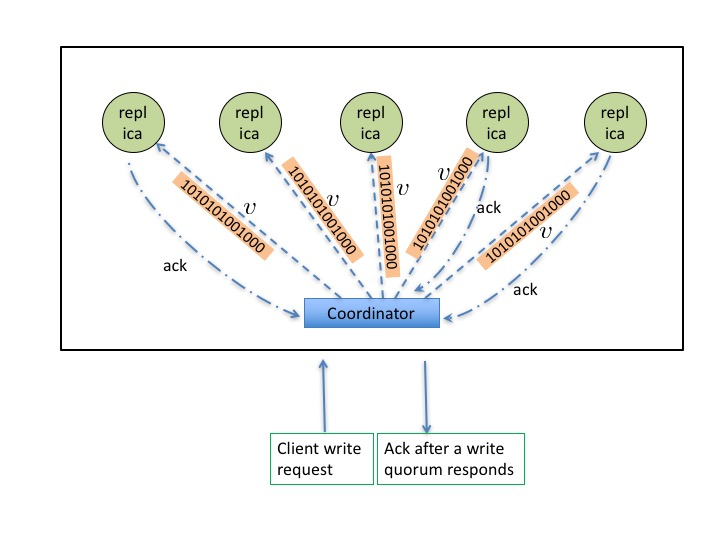
\includegraphics[width=\linewidth]{img/replication.jpg}
%		\caption{Cassandra stores the original value $v$.}
%		\label{fig:1}
%	\end{subfigure}
%	\hfill %%
%	\begin{subfigure}[b]{\columnwidth}
%		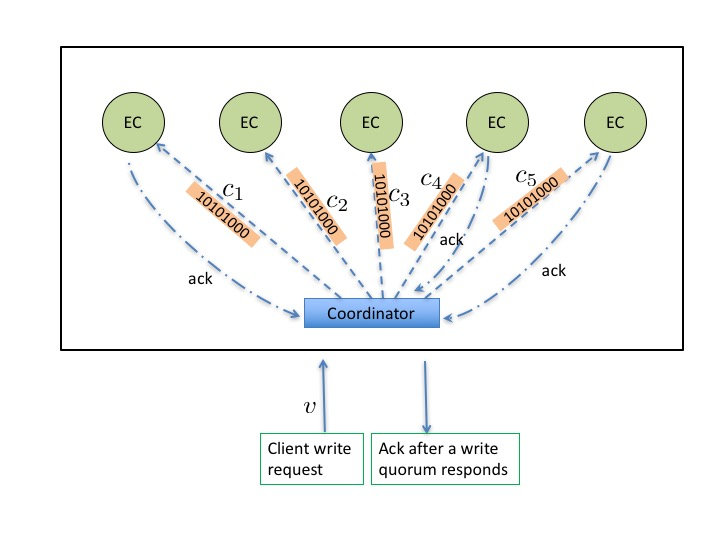
\includegraphics[width=\linewidth]{img/ec-code.jpg}
%		\caption{CassandrEAS only stores erasure-coded elements $c_i$'s.}
		%In TREAS and OREAS the erasure-coded elements of any value, e.g.,  $v$, is stored as  coded elements at separate servers.}
%		\label{fig:2}
%	\end{subfigure}
%	\caption{Illustration of Cassandra and CassandrEAS}
%\end{figure*}

% why EC?
% See motivaiton -- https://ipads.se.sjtu.edu.cn/_media/publications/cocytus_fast16.pdf
%\paragraph{Erasure Coding Storage Systems}
%\vspace*{3pt} \noindent \textbf{Erasure Coding Storage Systems}~~



	\section{Preliminaries}

\paragraph*{Erasure Coding Storage Systems}
Erasure coding (EC) is a space-efficient solution for data storage. 
EC has been traditionally used with great success for storage cost reduction in \textit{write-once, read-many-times} data stores (e.g., \cite{rashmi_fast15, dimakis2011survey, sathiamoorthy, HuaSimXu_etal_azure}). Recently there is an increasing interest in using EC in update-many-times, read-many-times data stores. As observed in \cite{Cocytus2016,GIZA2017}, with the advancement of hardware, it is possible to perform encoding/decoding in a real-time fashion.
EC also has the potential to significantly reduce network bandwidth, as well as for system maintenance (such as repairing failed servers).
Therefore, both information theory and system research communities have investigated the usage of erasure coding to reduce various kind of costs, e.g., \cite{dimakis2010network, rashmi2016ec, tamo2014family}.

% Prior Work
Two recent systems Cocytus \cite{Cocytus2016} and Giza \cite{GIZA2017} studied the applicability of erasure coding in other types of KV-stores. 
Giza~\cite{GIZA2017}, Microsoft's proprietary storage,  is a Fast-Paxos-based  multi-version cross-data center strongly consistent object store used in Microsoft's OneDrive storage system. Giza servers store erasure-coded elements instead of the original data to significantly reduce storage cost. 
Cocytus~\cite{Cocytus2016} is a master-based in-memory KV-store that guarantees strong consistency and reduces storage cost using erasure coding.  For each key,  value is erasure coded and the coded elements are stored among a subset of servers. In addition, the master server maintains a full copy of the value to provide high availability for read operations. 
%Cocytus uses a master and Giza uses consensus to coordinate servers.
As elaborated above, Cassandra's quorum-based design does not fit well with consensus protocol or master-based design.
%Their system designs are completely different from Cassandra, a quorum-based system. 
Therefore, we have to design a new EC-based protocol for using erasure coding in Cassandra.


%Theory community also shows interest in using erasure coding.
%EC-based algorithms for strongly consistent storage are also an active area of research in theory community, e.g., \cite{CadambeLMM17, SODA2016, LDS2017}.  %SODA\cite{SODA2016} described an algorithm to achieve optimal storage cost; however, pays higher write communication cost. 
%None of these algorithms have been integrated or implemented real-world systems. It is not clear how to adapt them into practical systems.

\paragraph*{Erasure Codes}
In this paper, we consider the optimal erasure codes. In particular, we adopt an $[n, l]$  linear Maximum Distance Separable (MDS) code ~\cite{verapless_book} over a finite field $\mathbb{F}_q$ to encode and store the value $v$ among the $n$ servers. Value is referred to a specific version of the data in our context. An $[n, l]$ MDS code has the property that any $l$ out of the $n$ coded elements can be used to recover (or decode) the original value $v$. 
For encoding, $v$ is divided\footnote{In practice, $v$ can be viewed as a byte array, which is divided into many stripes based on the choice of the code, various stripes are individually encoded and stacked against each other. We omit details of represent-ability of $v$ by a sequence of symbols of $\mathbb{F}_q$, and the mechanism of data striping, since these are fairly standard in the coding theory literature.} into $l$ elements $v_1, v_2, \ldots, v_l$ with each element having  size $\frac{1}{l}$ (assuming size of $v$ is $1$). The encoder takes the $l$ elements as input and produces $n$ coded elements $c_1, c_2, \ldots, c_n$ as output, i.e., $[c_1, \ldots, c_n] = \Phi^{(n,l)}([v_1, \ldots, v_l])$, where $\Phi^{(n, l)}$ denotes the encoder. For ease of notation, we simply write $\Phi^{(n, l)}(v)$ to mean  $[c_1, \ldots, c_n]$. The vector $[c_1, \ldots, c_n]$ is  referred to as the codeword corresponding to the value $v$. Each coded element $c_i$ also has  size $\frac{1}{l}$. In our scheme, we store \textit{one coded element} per key-value pair at each server. 

\remove{
\begin{algorithm*}[!ht]
	\begin{algorithmic}[2]
		{\footnotesize
			\begin{multicols}{2}
				\Statex /* at each reader  $r$ */
				\Operation{read}{} 
				%\State $wCounter\gets wCounter+1$
				\State $\tup{t_r, v} \gets \dagetdata{c}$
				\State $\daputdata{c}{ \tup{t_r,v}}$
				\State return $v$
				\EndOperation
				\Statex
				\Statex /* at each writer  $w$ */
				\Operation{write}{$v$} 
				%\State $wCounter\gets wCounter+1$
				%\State $t \gets $ machine time
				\State $t_w \gets (t, w)$ where $t$ is machine time at $w$
				\State $\daputdata{c}{\tup{t_w,v}}$
				\EndOperation
				
				\Statex
				\State /* helper functions for each $\pr_i$ */
				
				\Procedure{get-data}{}
				%	\State {\bf send} $(\text{{\sc query}},\rdr)$ to every server $s\in \bigcup_{cseq[i]}members(\qs_{cseq[i].conf})$
				\State {\bf send} $(\text{{\sc query-list}})$ to each  server $s$%\in \mathcal{S}$
				\State {\bf wait until}  receives $List_s$ from $\left\lceil \frac{n + k}{2}\right\rceil$ distinct servers%each server $s\in\srvSet_g$ s.t. $|\srvSet_g|=\left\lceil \frac{n + k}{2}\right\rceil$ 
				\State  $Tags_{*}^{\geq k} = $ set of tags that appears in  $k$ lists	\label{line:getdata:max:begin}
				\State  $Tags_{dec}^{\geq \ell} =$ tags appearing in $\ell$ lists with values
				\State  $t_{max}^{*} \leftarrow \max \{Tags_{*}^{\geq k} \}$; ~~~~~$t_{max}^{dec} \leftarrow \max \{ Tags_{dec}^{\geq \ell} \}$ \label{line:getdata:max:end}
				%\State  $t_{max}^{dec} \leftarrow \max \{ Tags_{dec}^{\geq \ell} \}$ \label{line:getdata:max:end}
				\If{ $t_{max}^{dec} \geq  t_{max}^{*}$} 
				\State  $v \leftarrow $ decode value for $t_{max}^{dec}$
				\EndIf
				%\State $List_M \triangleq \bigcup_{s \in \srvSet_g}  List_s$
				%$\State  $\forall t$, $List_M(t) \triangleq \{ (t, v): (t,v) \in List_M \}$  
				%\State $\forall t$, $T(t') \triangleq \{t: (t,v) \in List_M(t) \wedge t \geq t' \}$
				%\State $t_r \gets \max \{t : (t, *) \in List_M ~\wedge |List_M(t)| \geq k~\wedge |T(t)| \leq \delta \}$
				%\State $v_s\gets \text{decode from }  List_M(t_{r}))$
				\State {\bf return} $\tup{t^{dec}_{max},v}$
				\EndProcedure
				
				\Statex				
				
				\Procedure{put-data}{$\tup{\tg{},v})$}
				\State $\Coded = [(\tg{}, e_1), \ldots, (\tg{}, e_n)]$, $e_i = \Phi_i(v)$
				\State {\bf send} $(\text{{\sc write}}, \tup{\tg{},e_i})$ to each server $s_i$ %\in \mathcal{S}$
				\State {\bf wait until}  receives {\sc ack} from $\left\lceil \frac{n + k}{2}\right\rceil$ distinct servers
				\EndProcedure
				
			\end{multicols}
		}
	\end{algorithmic}	
	\caption{The steps for writers and readers in \oreas{}.}\label{alg:oreas-client}
\end{algorithm*}


\begin{algorithm*}[!ht]
	\begin{algorithmic}[2]
		{\footnotesize
			\begin{multicols}{2}
				\State{/* at each server $s_i$ */} %\in \mathcal{S}$}
				\State{\bf State variables:}%{ 										
				\Statex $List \subseteq  \mathcal{T} \times \mathcal{C}_s$, initially   $\{(t_0, \Phi_i(v_0))\}$
				
				\State
				\Receive{{\sc query-list}}{}%{$s_i,c_k$}
				\State Send $List$ to client $q$
				\EndReceive
				\State
				\Receive{{\sc put-data}, $\tup{\tg{},e_i}$}{}%{$s_i,c_k$}
				%{\color{blue}
				\State $\tg{max} = \max_{(t,c) \in List} \{t\}$
				
				\If{$\tg{} \geq \tg{max}$}   \label{line:treasmod:monotone:begin}
				\State /* Garbage collect old values */
				\State $List \gets List \backslash \{\tup{\tg{max},e_i}:  \tup{\tg{max},e_i} \in List\}$ 
				\State $List \gets List \cup \{\tup{\tg{},e_i}, \tup{\tg{max},\bot}\}$
				\Else
				\State $List \gets List \cup \{\tup{\tg{},\bot}\}$ \label{line:treasmod:monotone:end}
				\EndIf %}
				
				\State  Send {\sc ack} to client $q$
				\EndReceive
				
			\end{multicols}
		}
	\end{algorithmic}	
	\caption{The steps for server $s_i$ in  
		\oreas{}.}\label{alg:oreas-server}
\end{algorithm*}	
}

\paragraph*{Main Challenge}

The key challenge in an EC-based storage protocol that is compatible with quorum-based system is to handle concurrent operations.
To ensure high availability, the readers need to receive sufficient coded elements from the servers to be able to decode the version of the data that satisfies \textit{atomicity}. This issue becomes complicated in practice due to the following reasons: (i) there might be concurrent write operations that write different versions of the data simultaneously; (ii) servers and clients might crash so that the servers do not have enough coded element for a particular version; and (iii) messages might arrive in an arbitrary order due to the asynchrony assumption of the underlying network.
%If a read operation is concurrent with multiple write operations, then it is possible that the read is \textit{not} able to retrieve enough coded element to recover the original data. This situation becomes trickier with failures and asynchrony.

%There are two major ways of replicating data in KV-stores -- \emph{leader-based} or \emph{leaderless} strategy. Leader-based systems are often referred to as the primary-backup replication, with an appropriate consensus protocol like Paxos~\cite{PaxosSimple} or Raft~\cite{Raft} to elect a leader. Leaderless replication is mainly implemented based on quorum systems, and are used widely in NoSQL KV-stores.  The applicability of erasure coding in leader-based KV-stores has been recently explored in works like Cocytus \cite{Cocytus2016} and Giza \cite{GIZA2017}.  Our work is focused on using \textit{leaderless} strategy to provide strong consistency; hence, the technique is sufficiently different from prior leader-based storage systems. Moreover, we implement our algorithms in Cassandra, and show that CassandrEAS can handle typical NoSQL workload (using YCSB \cite{YCSB}) with low performance penalty.%, which was different from the in-memory \cite{Cocytus2016} and cross-datacenter systems \cite{GIZA2017}. 

%Cocytus~\cite{Cocytus2016} is a leader-based in-memory KV store that guarantees strong consistency. For each key, the ue is erasure coded and the coded elements are stored among a subset of servers. In addition, a primary server maintains a full copy of the value so as to provide high availability for read operations.  Giza~\cite{GIZA2017} is a leader-bsed cross-datacenter KV store that also guarantees strong consistency, and used in Microsoft's OneDrive storage system. Giza uses FAST-PAXOS (a variation of Paxos~\cite{PaxosSimple}) to elect the leader.
%The practicality of erasure-codes in Giza comes form the fact that an key-value pair is updated on average at most $4$ times during its life time.  

% Challenges
%\paragraph*{Challenges}
%\vspace*{3pt} \noindent \textbf{Challenges}~~
%On a high-level, erasure codes are more natural in leaderless systems than in leader-based systems. 

%%%%%%%%%%%%%%
%%%%%%% Maybe move Challenges to later??? %%%%%%%
%%%%%%%%%%%%%%

%\subsection{Challenges}
%Cassandra and other similar NoSQL KV-Stores  (e.g., \cite{Dynamo07,Riak}) use quorums to ensure strong consistency.  Specifically, they require the client (or a client proxy) to contact a group of servers. In replication-based protocols, the writer clients need to send \textit{identical} copies of data to all the servers in the quorum, which consumes unnecessary network bandwidth and storage space. The case of Cassandra is illustrated in Figure \ref{fig:1}. On the contrary, in EC-based protocols, clients only send or receive \textit{coded elements} from servers. This substantially reduces not only the storage overhead but also the communication overhead.

%The main challenge of using EC in quorum systems is efficient handling of read operations. %concurrent with write operations. To ensure high availability, the reader clients need to receive sufficient coded elements from the servers to be able to decode the original data (and complete the read operation). This issue becomes complicated in practice due to the following reasons: (i) there might be concurrent write operations, (ii) servers and clients might crash, and (iii) messages might arrive in an arbitrary order due to the asynchrony assumption of the underlying network.

\commentOut{++++++++++
\subsection{Main Contributions}

\paragraph*{Contributions: Protocol Design}
We propose a new EC-based distributed storage algorithm -- One-Round Erasure coding Atomic Storage (\oreas{}). Our algorithm tolerates network asynchrony and crash failures of any client and some fraction of servers, and achieve \textit{near-optimal storage cost}.
%Similar to the design of vanilla Cassandra, if clocks drift significantly, then \oreas{} might violate strong consistency. On the contrary, \treasmod{} ensures strong consistency at all time, but suffers an extra round of delay due to the usage of logical timestamp.
%We propose a new EC-based storage scheme. If we use logical timestamps for each operation, then it requires two rounds to complete an operation, namely \treasmod. In this case, strong consistency is guaranteed at all time. On the other hand, if we use physical timestamps (i.e., machine time), then it only requires one round to complete an operation, namely \oreas. Similar to the replication-based protocol in Cassandra, \oreas{} might violate strong consistency if clocks at servers drift significantly.
\oreas{} has two benefits listed below. Let $\delta$ represent the maximum number of writes concurrent with any read.
\begin{itemize}
	\item The storage cost at each server is $\frac{B}{ \lceil\frac{\delta+1}{k}\rceil}$ bits for storing $B$-bit data. The new storage scheme is at least as efficient as the common EC-based protocols where each server stores codeword symbols for $\delta$ versions, e.g., \cite{ARES:ICDCS:2019}. Furthermore, for certain parameters of $\delta,k$, the new scheme can be up to twice as storage-efficient. For example, if we use an $[n = 5, k = 3]$ MDS code, the storage cost is simply  $1.67$ per unit of data, instead of $5$ as in the case of vanilla Cassandra.
	
	%\item An $[n, k]$ erasure code splits the value $v$ of size $1$ unit into $k$ elements, each of size $\frac{1}{k}$ units, creates $n$ {\em coded elements}, and stores one coded element per server. The size of each coded element is also $\frac{1}{k}$ units, and thus the total storage cost across the $n$ servers is $\frac{n}{k}$ units. For example, if we use an $[n = 5, k = 3]$ MDS code, the storage cost is simply  $1.67$ per unit of data, instead of $5$ as in the case of replication-based algorithms, such as ABD.
	
	
%	$B/\lceil \frac{l}{\delta}\rceil$ bits. Since $\frac{\delta}{l} \geq 1/\lceil \frac{l}{\delta}\rceil,$ the new storage scheme is at least as efficient as the common EC-based protocols where each server stores codeword symbols for $\delta$ versions, e.g., \cite{ARES:ICDCS:2019}. Furthermore, for certain parameters of $\delta,l$, the new scheme can be up to twice as storage-efficient. %as previous EC-based protocols. 
	
	\item In the new scheme, as in most replication-based approaches (such as the well-known replication-based algorithm by Attiya, Bar-Noy, and Dolev~\cite{ABD96} and Dynamo-style quorum systems \cite{Cassandra2010,Dynamo07,pbs-vldb2012}),  each server stores \underline{exactly one version of the data.} This is contrast to previous EC-based protocols (e.g., \cite{CadambeLMM14}) where $\delta$ versions of the data are stored at the server. 
\end{itemize}

%(which we refer to as ABD)

\paragraph*{Contributions: System}

We implement \treasmod{} and \oreas{} into Cassandra \cite{Cassandra2010}, namely CassandrEAS.
We pick Cassandra to be our base system due to its popularity and wide applications.
Cassandra adopts a practical partial quorum approach (or Dynamo-style quorum) \cite{pbs-vldb2012} for replicating data.
We replace its replication mechanism by our new EC-based protocols.
We try to make minimum modification to the original Cassandra codebase, and Cassandra users can call Cassandra's original read and write API directly \textit{without} knowing the details of the algorithm.\footnote{Our algorithm does not support transaction; hence, those transaction-related APIs are not supported.} 
To the best of our knowledge, this is the first implementation in NoSQL KV-Store that uses erasure coding.\footnote{We will release our code on Github once the paper is accepted in hope that stimulate more discussion and evaluation on using erasure codes in similar systems.} 

For evaluation, we deploy CassandrEAS in Google Cloud Platform (GCP) and conduct extensive experiments using the Yahoo! Cloud Service Benchamarking (YCSB) workload generator \cite{YCSB:2010}. YCSB is a realistic tool used to benchmark many KV-stores.
The implementation is discussed in Section \ref{s:implementation} and we present evaluation results in Section \ref{s:evaluation}.

++++++++++++=}





% prior work. We can talk about key-value systems that are completely different and does not use quorums (so we don't have to worry about comparing) or large systems like Giza, a proprietary system. What do you think we take a motivation as below.

% our contribution



% Kishori's guideline
%a)  is it possible to even use EC code based key-value in Cassandra, which is a super popular key-value, store to reduce storage cost? 
%b) But wait a minute, Cassandra wants strong consistency, which is not so easy with failure, asynchrony and EC,  however, it uses replication and quorum for now but might be possible to use EC with quorums
%c) Thankfully, we created a simple algorithm with might be possible to put into Cassandra.
%d) With lots of pain we managed to implement it in Cassandra, and got some interesting results.
%e) Let me describe the results to you now






    \subsection{Model and Definitions}\label{model}

A shared atomic storage (or atomic KV-store) can be emulated
by composing individual atomic objects. Therefore, we aim
to implement \nn{a single} atomic read/write memory object. %on a set of servers.
A read/write object takes a value from a set $\valSet$. 
We assume a system consisting of three distinct sets of processes: 
a set $\wSet$ of writers, a set $\rdSet$ of readers and  $\srvSet$, a set of servers. 
 Servers host data elements (replicas or encoded data fragments).
Each writer is allowed to modify the value of a shared object, and each reader is allowed to obtain 
the value of that object. 
Processes communicate via \myemph{messages} through 
\myemph{asynchronous}, but \myemph{reliable} channels. 
%%Let $\idSet = \cSet\cup\reconSet\cup\srvSet$. 
%In a read/write object implementation, we assume that the object may take a value from a set $\valSet$. 
%Each writer is allowed to modify the value of the object, and each reader is allowed to obtain 
%the value of the object. Servers host data elements (replicas or encoded data fragments).
%%maintain encoded elements of the redundant object.
%
%We assume an \myemph{asynchronous} environment, where processes communicate
%by exchanging messages. The writer, any subset of readers, and up to 
%$f$ servers may \myemph{crash} without any notice.
%\ares{} allows the set of server host to be modified during the course of an execution for 
%masking transient or permanent failures of servers and preserve the longevity of the service.  
%\kmk{In the paper, we are interested only  in the fair executions of any algorithm.}


%we can formally define a quorum system $\quorums{c}$, with $c\in\confSet$, as follows:
%Consider a configuration identifier $c$.
%We define as $\servers{c}=\bigcup_{Q\in\quorums{c}} Q$ the set of servers that belong in the quorums
%f a quorum system $\quorums{c}$. 
%We refer to a server $s$ as a \myemph{member} of a configuration $c$ if $s\in \servers{c}$.

%
%\paragraph{Notations and Definitions}  We denote by $\mathcal{W}$, $\mathcal{R}$ and $\mathcal{S}$,  the set of writers, readers and servers, respectively.
%We denote by $\confSet$ the set of possible configurations of the systems. A configuration $c \in \confSet$ has a unique the configuration identifier   $c.conf$; a set of servers $c.servers$, such that, $c.Servers \subseteq \mathcal{S}$,
%$cseq[i].status\in\{F,P\}$, the pending or finalized status 

%The writer process $w$ may invoke write operations on the atomic object 
%by calling the $\act{write}(v)$ function whereas each reader may invoke 
%a read operation by calling the $\act{read}$ function. Each write event 
%returns an acknowledgement when successfully carried-out, whereas each read 
%operation returns the value of the atomic object. We assume that an 
%

\myparagraph{Executions.} 
%An algorithm $A$ is a collection of processes, where process $A_p$
%is assigned to processor $p\in\idSet\cup\srvSet$. The \textit{state}, of a process $A_\pr$ is determined over a
%set of state variables, and the state $\state$ of $A$ is a vector that contains the state of
%each process. Each process $A_\pr$ implements a set of actions. When an action $\acts{}$ occurs 
%it causes the state of $A_\pr$ to change, say from 
%some state $\state_p$ to some different state $\state_p'$. We call the triple $\tup{\state_p, \acts{}, \state_p'}$
%as a \textit{step} of $A_\pr$. Algorithm $A$ performs a step, when some process $A_\pr$ performs a step.
%: (i) receives a
%message, (ii) performs local computation, (iii) sends a message. 
%Each such action
%causes the state at $p$ to change. 
An \textit{execution} of an algorithm $A$  is an alternating sequence of states
and actions of $A$ starting with the initial state and ending in a state. 
An execution $\EX$ is \textit{well-formed} if any process invokes one operation
at a time and it is \textit{fair} if enabled actions perform a step infinitely often. In the rest of the paper 
we consider executions that are fair and well-formed. A process
$\pr$ \textit{crashes} in an execution if it stops taking steps; otherwise $p$ is \textit{correct} or \textit{non-faulty}.


\myparagraph{Write and Read Operations.}
An implementation of a read or a write operation contains an \textit{invocation} action  and a \textit{response} action (such as a
	return from the procedure). An operation $\op$ is \textit{complete} in an execution, if it
	contains both the invocation and the \textit{matching} response actions for $\op$; otherwise $\op$
	is \textit{incomplete}. 
	We say that an operation $\op$ \textit{precedes} an operation $\op'$ in an execution $\EX$,
	denoted by $\op\bef\op'$, if the response step of $\op$ appears before the invocation
	step of $\op'$ in $\EX$. Two operations are \textit{concurrent} if neither precedes the other.
	An implementation $A$ of a read/write object satisfies the atomicity property
	if the conditions of Lemma 13.16 in  \cite{Lynch1996} holds. 
	
\myparagraph{Storage and Communication Costs.} 
\remove{We are interested in the \myemph{complexity} of each
read and write operation. The complexity of each operation $\op$ invoked by a process 
$\pr$, is measured with respect to three metrics, during the interval between the invocation 
and the response of $\op$: (i) \myemph{communication round-trips}, accounting the number of messages 
sent during $\op$, (ii) \myemph{storage efficiency} \nn{(storage cost)}, accounting the maximum storage requirements for 
any single object at the servers during $\op$, and  (iii) \myemph{message bit complexity} \nn{(communication cost)}
which measures the size of the messages used during $\op$. 
}
We define the total storage cost as the size of the
data stored across all servers, at any point during the execution of the algorithm. The
communication cost associated with a read or write operation is the size of the total data that
gets transmitted in the messages sent as part of the operation. We assume that metadata,
such as version number, process ID, etc. used by various operations is of negligible size, and therefore,  ignore in the calculation of storage and communication cost. Further, we normalize
both the costs with respect to the size of the value v; in other words, we compute the costs
under the assumption that v has size 1 unit.
%\lewis{This is repetitive? Didn't we already discuss this before? Second paragraph of this section.}
%\blue{Yes, now removed}

 
\myparagraph{Quorum system}. We define our quorum system, $\mathcal{Q}$, to be the set of all subsets of $\mathcal{S}$ that have at least $\frac{n+k}{2}$ servers. We refer to the members of $\mathcal{Q}$, as quorum sets and they satisfy the following property.

\begin{lemma}
For any $k$,  $1 \leq k \leq n -2f$. (i) If $Q_1$ ,$Q_2 \in \mathcal{Q}$,
then $|Q_1 \cap Q_2 | \geq k$. (ii) If the number of failed servers is
at most $f$ , then $Q$ contains at least one quorum set $Q$ of
non-failed servers.
\end{lemma}
%\myparagraph{Storage and Communication Cost.} We define the total storage cost as the size of the
%data stored across all servers, at any point during the execution of the algorithm. The
%communication cost associated with a read or write operation is the size of the total data that
%gets transmitted in the messages sent as part of the operation. We assume that metadata,
%such as version number, process ID, etc. used by various operations is of negligible size, and
%is hence ignored in the calculation of storage and communication cost. Further, we normalize
%both the costs with respect to the size of the value v; in other words, we compute the costs
%under the assumption that v has size 1 unit.

%A communication round-trip
%(or simply round) is more formally defined in the following definition that appeared in \cite{CDGL04,GNS09,GNS08}:

%\begin{definition}\label{def:com}
%Process $p$ performs a communication round during operation $\op$ 
%if all of the following hold:
%\begin{enumerate}
%   \item $p$ sends request messages that are a part of $\op$ 
%         to a set of processes,
%	\item any process $q$ that receives a request message from $p$ for 
%         operation $\op$, replies
%% to it with an acknowledgment 
%%         message, at the first possible convenience and 
%without delay, i.e. without waiting for any other messages before 
%replying to $\op$.
%   \item when process $p$ receives ``enough'' replies it 
%terminates the round
%%, orreturns or repeats a communication round
%         %then makes a local decision about termination of the phase.
%\end{enumerate}
%\end{definition}
%
%At the end of a communication round process $\pr$ may complete $\op$
%or start a new round. Operation $\op$ is \myemph{fast} \cite{CDGL04} if it completes after 
%its first communication round; an implementation is fast if in each execution
%all operations are fast.

\myparagraph{Liveness of operations.} We require algorithms to satisfy certain liveness properties, specifically, in every fair execution that satisfies certain restrictions in terms of the number of failed nodes, we require every operation by a non-faulty client 
completes eventually, irrespective of the behavior of other clients.  
Although most replication-based based atomic memory algorithm guarantee liveness as long as certain no of servers remain 
non-faulty.  Unfortunately, certain lower bounds on the storage-cost of erasure-coded atomic memory algorithm in the presence of faulty clients ~\cite{cadambe2016information, SCCK15}. As a result, to  circumvent this restriction many authors assume certain restricting 
assumption.  CASGC, ORCAS-A and ORCAS-B~\cite{DGL08} assume a bound on the number of concurrent operation. In the same vein, \treasmod{} assumes a known bound on the number of concurrent writes with a read to achieve liveness. 


	\section{\treasmod: Storage-optimized two-round algorithm}\label{sec:treasmod}
The pseudo-code for  ~\treasmod{} is presented in  Alg.~\ref{fig:treasmod}. 
\treasmod{} is parameterized by the number of servers $n$, the quorum intersection size $k$, and the degree of concurrency that can be tolerated $\delta$. Note that $k$ does not represent the dimension of the code here. 
%
The algorithm uses an MDS code, with encoding function $\Phi^{(n,\ell)}: \mathbb{F}^{\ell} \rightarrow \mathbb{F}^{n}$ where, $\mathbb{F}$ represents the finite field over which encoding is performed, $n$ represents the length of the code, and $\ell = {\lceil \frac{k}{\delta+1} \rceil} $ represents the dimension of the code. 

\treasmod{}  shares some similarities with ABD \cite{ABD96} as well as ~\treas~\cite{NicolaouC0KML19}. Specifically, in \treasmod{}, like ~\treas{}, erasure coding is used, and each server stores a list of all the tags that it receives in the execution; even if the coded element corresponding to a tag $t$, logical timestamp, is garbage collected, the server stores a tuple of the form $(t, \bot)$. However, unlike ~\treas{}, in \treasmod{} each server stores only coded element, similar to ABD~\cite{ABD96}. When a new tag-coded-element pair arrives  at a server, if the tag is larger than the highest locally stored tag $\tau_{max}$, then the server simply replaces the stored coded element by the newly arriving coded element; however the server will continue to store a tuple of the form $(\tau_{max},\bot)$.

While in~\treas{}, each server stores $\delta+1$ coded elements of a code with dimension $k$, in \treasmod{}, each server stores \emph{one} coded element of dimension ${\lceil \frac{k}{\delta+1} \rceil}$. Since the size of each coded element is effectively a fraction $\frac{1}{k}$ the size of the value, the server storage cost in~\treas{} normalized by the size of the object is $\frac{\delta+1}{k},$ whereas the storage cost of \treasmod{} is $\frac{1}{\lceil \frac{k}{\delta+1}\rceil}$  since 
$  \frac{\delta+1}{2 k} < \frac{1}{\lceil \frac{k}{\delta+1}\rceil} \leq \frac{\delta+1}{k}$
the storage cost of \treasmod{} is no worse than the storage cost of ~\treas{}, and can be up to twice as efficient. For instance, if we have $n=9$ servers, and we use quorums of size $6$ so that $k=3$, for a concurrency of $\delta=1$, the storage cost of ~\treas{} is $2/3$, whereas the cost of \treasmod{} is $\frac{1}{2}.$ For the same system, if quorums of size $7$ are used, and a concurrency can be bounded by $\delta=3$, then the storage cost of~\treas{} is $4/5=0.8$ whereas \treasmod{} has a storage cost of $1/2=0.5$. 


% However, liveness is  guaranteed under the assumption that the number of write operations concurrent with a read  operation is at most $\delta$. The precise definition of concurrency depends on the algorithm itself, and appears later in this section. The \treasmod{}~algorithm has significantly reduced storage and communication cost, compared to replication, when $\delta$ is limited.
%Expressing an atomic algorithm in terms of the DAP primitives serves multiple purposes.
%First, describing an algorithm according to template algorithm $A_1$  allows one to proof
%that the algorithm is \textit{safe} (atomic) 
%% it enables ease of reasoning about the safety of the algorithm  
%% given that atomicity holds if 
%by just showing that the appropriate DAP properties hold, and the algorithm is \textit{live} if the 
%implementation of each primitive is live. 
%Secondly, the safety and liveness proofs for more complex algorithms (like \ares{} in Section \ref{sec:ares}) % algorithm  
%become easier as one may reason on the DAP properties that are satisfied by the primitives used,
%without involving the underlying implementation of those primitives. 
%Moreover, describing a reconfiguration algorithm using DAPs, provides the flexibility 
%to vary the  implementations DAPs from configuration to configuration, as long as the DAPs satisfy certain  properties. 
%%
%%is easier where  complex operations like reconfiguration is done, where the implementation of data-access primitives can vary from one configuration to another,  while
%%hiding the details of the underlying atomic algorithm implementation. 
%%
%%
%%As we show 
%%In Section \ref{sec:algorithm}, we discuss how \ares{} may change the primitives mechanisms
%%such data access primitives allows us to design 
%%a reconfigurable atomic storage service that can utilize different atomic implementation 
%%in each established configuration without affecting the safety guarantees of the service.
%%Such approaches can adapt to the configuration design, and vary the performance of the service
%%based on the environmental conditions.
%% In other words, ABD \cite{ABD96} can be used for 
%%maximum fault tolerance and when majority quorums are used, whereas fast algorithms 
%%similar to the ones presented in \cite{CDGL04, FNP15}, could be used in configurations 
%%that satisfy the appropriate participation bounds. 
%
%{\color{blue}

A tag $\tg{}$ is defined as a pair $(z, w)$, where $z \in \mathbb{N}$ and $w \in \mathcal{W}$, an ID of a writer.
Let $\mathcal{T}$ be the set of all tags.
Notice that tags could be defined in any totally ordered domain and given that this domain is countably infinite, then 
there can be a direct mapping to the domain we assume. 
% and we denote by  $\mathcal{T}$  the set of all possible tags. 
For any  $\tg{1}, \tg{2} \in \mathcal{T}$, where $
\tau_i = (z_i, w_i)$,  we define  $\tg{2} > \tg{1}$ if $(i)$ $\tg{2}.z > z_1$ or $(ii)$ $z_2 = z_1$ and $w_2 > w_1$.

Each server $s_i$ stores one  state variable,  $List$,  which is a set of up to $(\delta + 1)$  (tag, coded-element) pairs. Initially the set at $s_i$ contains a single element, $List = \{ (t_0,  \Phi_i(v_0)\}$.  
 A read operation at a client is implemented based on the \act{get-data} and \act{put-data} steps; and a write operation is based on the \act{get-tag} and \act{put-data} steps. Below we describe these steps in more detail.
%\sout{Below we describe the implementation of the DAPs.} 
 
%\lewis{What is DAPs?}
%
%				At a high-level, the algorithm (see Fig.~\ref{fig:casopt}) is a natural generalization of the $ABD$ algorithm accounting for the fact that we use MDS codes.

%\kishori{
$\dagettag{c}$: A  client,  during the execution of a  $\dagettag{c}$ primitive, queries all the servers in $\mathcal{S}$ for the highest tags in their  $Lists$, and awaits responses from $\left\lceil \frac{n+k}{2} \right\rceil$ servers.
% with $k \geq \frac{2n}{3}$. 
A server upon receiving the {\sc get-tag} request, 
responds to the client with the highest tag, as $\tg{max} \equiv \max_{(t,c) \in List}t$. 
Once the client receives the tags from $\left\lceil \frac{n+k}{2} \right\rceil$ servers,  it selects  the highest  tag $t$ and returns it . 
%}

%\kishori{
$\act{put-data}(\tup{t_w, v})$: During the  execution of the primitive  $\act{put-data}(\tup{t_w, v})$,  a client 
% computes the coded elements for each of the $n$ servers, and 
sends the  pair  $(t_w, \Phi_i(v))$ to each server $s_i\in\mathcal{S}$.  
When a server $s_i$ receives a message $(\text{\sc put-data}, t_w, c_i)$ , it adds the pair in its local $List$, 
trims the pairs with the smallest tags exceeding the length $(\delta+1)$ of the $List$ , and replies 
with an ack to the client.
%
%Every time a $(\text{\sc put-data}, t_w, c_i)$  message arrives at a server $s_i$, 
%from a writer, 
%the pair gets added to the $List$. As the size of the $List$ at each $s_i$ is bounded by $(\delta+1)$, then following an insertion in the $List$, $s_i$ trims the coded-elements associated with the smallest tags. 
In particular, $s_i$ replaces the coded-elements of the older tags with $\bot$, and maintains only the coded-elements associated with the 
$(\delta+1)$ highest tags in the $List$ (see Line Alg.~\ref{fig:treasmod:server}:\ref{line:treasmod:monotone:begin}-\ref{line:treasmod:monotone:end}).
%which is then garbage collected to keep tag and coded-element pairs of the highest  $(\delta+1)$ tags, and by replacing the coded-elements of the older tags with $\bot$,  a symbol that signifies garbage-collected coded-elements.
The client completes the primitive operation after getting acks from $\left\lceil \frac{n+k}{2} \right\rceil$ servers.
%}

%\kishori{
$\dagetdata{c}$:	A  client, during the execution of a  $\dagetdata{c}$ primitive, queries all the servers in $\mathcal{S}$ for their  local variable $List$, and awaits responses from $\left\lceil \frac{n+k}{2} \right\rceil$ servers. Once the client receives $Lists$ from $\left\lceil \frac{n+k}{2} \right\rceil$ servers,  it selects the highest  tag $t$, such that: $(i)$ its corresponding value $v$ is decodable from the coded elements in the lists; and $(ii)$ $t$ is the highest tag seen from the responses of at least $k$ $Lists$ 
(see lines Alg.~\ref{fig:treasmod}:\ref{line:getdata:max:begin}-\ref{line:getdata:max:end}) and returns the pair $(t, v)$. 
Note that in the case where anyone of the above conditions is not satisfied the corresponding read operation does not complete.
%}

The main technical aspect in which {\treasmod} differs with, in terms of correctness, in comparison with ~\treas{} is the liveness proof. We argue that despite the changes, {\treasmod} guarantees termination of every read operation whose concurrency is below $\delta$.
%} 

%\remove{
\begin{algorithm*}[!ht]
				\begin{algorithmic}[2]
					{\footnotesize
					\begin{multicols}{2}
				
				\Statex /* at reader $r$ */
				\Operation{read}{} 
				%\State $wCounter\gets wCounter+1$
				\State $\tup{t_r, v} \gets \dagetdata{c}$
				\State $\daputdata{c}{ \tup{t_r,v}}$
				\State return $v$
				\EndOperation
				\Statex
				\Statex /* at writer $w$ */
				\Operation{write}{$v$} 
				%\State $wCounter\gets wCounter+1$
				\State $t_{max} \gets \dagettag{c}$
				\State $t_w \gets (t_{max}.z+1, w)$
				\State $\daputdata{c}{\tup{t_w,v}}$
				\EndOperation
							\State{ at each process $\pr_i\in\idSet$}
	
							\Statex
							\Procedure{get-tag}{}
							%	\State {\bf send} $(\text{\act{query}},\rdr)$ to every server $s\in \bigcup_{cseq[i]}members(\qs_{cseq[i].conf})$
							\State {\bf send} $(\text{{\sc query-tag}})$ to each  $s\in \mathcal{S}$
							\State {\bf until}  receives $\tup{t_s,e_s}$ from $\left\lceil \frac{n + k}{2}\right\rceil$ servers
							\State $t_{max} \gets \max(\{t_s : \text{ received }  \tup{t_s,v_s} \text{ from } s \})$ \label{line:gettag:max}
							\State {\bf return} $t_{max}$
							\EndProcedure
							
							\Statex
							
							\Procedure{get-data}{}
							%	\State {\bf send} $(\text{{\sc query}},\rdr)$ to every server $s\in \bigcup_{cseq[i]}members(\qs_{cseq[i].conf})$
								\State {\bf send} $(\text{{\sc query-list}})$ to each  $s\in \mathcal{S}$
								\State {\bf until}  receives $List_s$ from each server $s\in\srvSet_g$ s.t. $|\srvSet_g|=\left\lceil \frac{n + k}{2}\right\rceil$ 
								\State  $Tags_{*}^{\geq k} = $ set of tags that appears in  $k$ lists	\label{line:getdata:max:begin}
								\State  $Tags_{dec}^{\geq \ell} =$ tags appearing in $\ell$ lists with values
								\State  $t_{max}^{*} \leftarrow \max Tags_{*}^{\geq k} $
                                \State  $t_{max}^{dec} \leftarrow \max Tags_{dec}^{\geq \ell} $ \label{line:getdata:max:end}
								\If{ $t_{max}^{dec} \geq  t_{max}^{*}$} \label{line:getdata:max:equal}
								    \State  $v \leftarrow $ decode value for $t_{max}^{dec}$
								\EndIf
								%\State $List_M \triangleq \bigcup_{s \in \srvSet_g}  List_s$
								%$\State  $\forall t$, $List_M(t) \triangleq \{ (t, v): (t,v) \in List_M \}$  
								%\State $\forall t$, $T(t') \triangleq \{t: (t,v) \in List_M(t) \wedge t \geq t' \}$
								%\State $t_r \gets \max \{t : (t, *) \in List_M ~\wedge |List_M(t)| \geq k~\wedge |T(t)| \leq \delta \}$
								%\State $v_s\gets \text{decode from }  List_M(t_{r}))$
								\State {\bf return} $\tup{t^{dec}_{max},v}$
							\EndProcedure
							
							\Statex				
							
							\Procedure{put-data}{$\tup{\tg{},v})$}
								\State $\Coded = [(\tg{}, e_1), \ldots, (\tg{}, e_n)]$, $e_i = \Phi_i(v)$
								\State {\bf send} $(\text{{\sc put-data}}, \tup{\tg{},e_i})$ to each $s_i \in \mathcal{S}$
								\State {\bf until}  receives {\sc ack} from $\left\lceil \frac{n + k}{2}\right\rceil$ servers
							\EndProcedure
							%\EndPart
							
							
							
%							\Part{write($v$)}\EndPart
%							\Part{\underline{\GetTag}} {
%								\State  Send  $(\QueryTag)$ to all servers $\mathcal{S}$.
%								\State  Await responses from majority
%								\State  Select the max tag  $t^*$
%							}\EndPart
%							\Statex
%							\Part{\underline{\PutData}} {
%								\State $t_w = (t^{*}.z + 1, w)$.  
%								\State $\Coded = [(t_w, c_1), \ldots, (t_w, c_n)]$, $c_i = \Phi_i(v)$
%								\State Send  $(\CodedElementTag, \Coded)$ to all servers $\mathcal{S}$.
%								\State Terminate after $\left\lceil \frac{n + k}{2}\right\rceil$ acks
%							}	\EndPart
							
%							\Statex
%							\Part{read}\EndPart
%							\Part{\underline{\GetData}} {
%								\State  Send $(\QueryList)$ to all servers $\mathcal{S}$.
%								\State  Wait for $\left\lceil \frac{n+k}{2}\right\rceil$ $Lists$ 
%								\State  Select the max tag, $t_r$, the corresponding value, $v_r$, is decodable using the $Lists$; additionally   $t_r$ is among the highest distinct $\delta$ tags received in any $Lists$.
%							}\EndPart	
%							\Statex
%							\Part{\underline{\PutData}} {
%								\State $\Coded = [(t_r, c_1), \ldots, (t_r, c_n)]$, $c_i = \Phi_i(v_r)$
%								\State Send $(\CodedElementTag, \Coded)$ to all servers $\mathcal{S}$.
%								\State Wait for $\left\lceil \frac{n + k}{2}\right\rceil$ acks
%								\State Return $v_r$
%							}	\EndPart
%							
%							
					\end{multicols}
				}
				\end{algorithmic}	
				\caption{The reader/writer client-side steps for implementing \treasmod{}.}\label{fig:treasmod}
				\vspace{-1em}
	\end{algorithm*}
		

	\begin{algorithm*}[!ht]
	\begin{algorithmic}[2]
		{\footnotesize
		\begin{multicols}{2}
				\State{at each server $s_i \in \mathcal{S}$}
				\Statex
				\State{\bf State Variables:}%{ 										
					%\Statex $(t_{loc}, v_{loc}) \in \mathcal{T} \times {\mathcal V}$, initially   $(t_0, v_0)$
					%\Statex $status \in \{active, repair\}$, initially $active$
					\Statex $List \subseteq  \mathcal{T} \times \mathcal{C}_s$, initially   $\{(t_0, \Phi_i(v_0))\}$
				%}\EndPart
			
			\Statex
			\Receive{{\sc query-tag}}{}
				\State $\tg{max} = \max_{(t,c) \in List}t$
				\State Send $\tg{max}$ to $q$
			\EndReceive
			\Statex
	
			
			\Receive{{\sc query-list}}{}
				\State Send $List$ to $q$
			\EndReceive
\State
			\Receive{{\sc put-data}, $\tup{\tg{},e_i}$}{}
			%{\color{blue}
				\State $\tg{max} = \max_{(t,c) \in List}t$

				\If{$\tg{} \geq \tg{max}$}   \label{line:treasmod:monotone:begin} 
					\State $List \gets List \backslash \{\tup{\tg{max},e_i}:  \tup{\tg{max},e_i} \in List\}$ 
					\State $List \gets List \cup \{\tup{\tg{},e_i}, \tup{\tg{max},\bot}\}$
				\Else
					\State $List \gets List \cup \{\tup{\tg{},\bot}\}$ \label{line:treasmod:monotone:end}
                                   \EndIf %}

								\State  Send {\sc ack} to $q$
			\EndReceive
			
%				\Statex
%				\Part {\underline{\GetTagResp,recv $\QueryTag$ from writer $w$}} {
%					%\If{ $status = active$ }
%					\State $t^* = \max_{(t,c) \in List}t$
%					\State Send $t^*$ to $w$
%					\Statex %\EndIf
%				}\EndPart
%				%										\Statex
%				\Part {\underline{\GetDataResp, recv $\QueryList$ from reader $r$}} {
%					%\If{ $status = active$ }
%					\State Send  $List$ to $r$
%					%\EndIf
%				}\EndPart
%				%	
%				\Statex
%				\Part{ \underline{\PutDataResp, recv $\CodedElementTag, (t, c_i)$ from $p$ }}{
%					%\If{$status = active$}
%					\State $List \leftarrow List \cup \{ (t, c_i)  \}$ 
%					\If{ $|List| > \delta + 1$ } 
%					\State  Retain the (tag, coded-element) pairs for the $\delta +1 $ highest tags in $List$, and delete the rest.
%					\EndIf 
%					\State  Send ack to $p$.
%					%\EndIf
%					
%				}\EndPart
				\end{multicols}
			}
	\end{algorithmic}	
	\caption{The response protocols at  any server $s_i \in {\mathcal S}$ in  
					\treasmod{} for client requests.}\label{fig:treasmod:server}
					\vspace{-1em}
\end{algorithm*}	
%}

\myparagraph{Safety and Liveness  properties}\label{sec:treas_safety_liveness}
Now we state the safety  and liveness properties of \treasmod.
%Due to lack of space the proofs are deferred for a later extended version of the paper.

\remove{						
 \begin{lemma}\label{casflex:data-access:consistent}
The data-access primitives, i.e., $\act{get-tag}$, $\act{get-data}$ and $\act{put-data}$ primitives, implemented in the \treasmod{} algorithm satisfy the consistency properties.
\end{lemma}
}

\remove{
\begin{proof}
As mentioned above we are concerned with only configuration $c$, and therefore, in our proofs we will be concerned with only one
configuration. Let $\alpha$ be some execution of \treasmod{}, then we consider two cases for $\pi$ for proving property $C1$:  $\pi$ is a  $\act{get-tag}$ operation, or $\pi$ is a $\act{get-data}$ primitive. 

 %\item[ C1 ]  If $\phi$ is a  $\daputdata{c}{\tup{\tg{\phi}, v_\phi}}$, for $c \in \confSet$, $\tg{1} \in\tsSet$ and $v_1 \in \valSet$,
 %and $\pi$ is a $\dagettag{c}$ (or a $\dagetdata{c}$) 

 %that returns $\tg{\pi} \in \tsSet$ (or $\tup{\tg{\pi}, v_{\pi}} \in \tsSet \times \valSet$) and $\phi$ completes before $\pi$ in $\EX$, then $\tg{\pi} \geq \tg{\phi}$.
Case $(a)$: $\phi$ is   $\daputdata{c}{\tup{\tg{\phi}, v_\phi}}$ and  $\pi$ is a $\dagettag{c}$ returns $\tg{\pi} \in \tsSet$. Let $c_{\phi}$ and $c_{\pi}$ denote the clients that invoke $\phi$ and $\pi$ in $\alpha$. Let $S_{\phi} \subset \mathcal{S}$ denote the set of $\left\lceil \frac{n+k}{2} \right \rceil$ servers that responds to $c_{\phi}$, during $\phi$. Denote by $S_{\pi}$ the set of $\left\lceil \frac{n+k}{2} \right \rceil$ servers that responds to $c_{\pi}$, during $\pi$.  Let $T_1$ be a point in execution $\alpha$ 
after the completion of $\phi$ and before the invocation of $\pi$. Because $\pi$ is invoked after $T_1$, therefore, at $T_1$ each of the servers in $S_{\phi}$ contains $t_{\phi}$ in its $List$ variable. Note that, once a tag is added to $List$, it is never removed. Therefore, during $\pi$, any server in $S_{\phi}\cap S_{\pi}$ responds with $List$ containing $t_{\phi}$ to $c_{\pi}$. Note that since  $|S_{\sigma^*}| = |S_{\pi}| =\left\lceil \frac{n+k}{2} \right \rceil $ implies
				 $| S_{\sigma^*} \cap S_{\pi} | \geq k$, and hence $t^{dec}_{max}$ at $c_{\pi}$, during $\pi$ is at least as large as $t_{\phi}$, i.e., $t_{\pi} \geq t_{\phi}$. Therefore, it suffices to to prove our claim with respect to the tags and the decodability of  its corresponding value.


Case $(b)$: $\phi$ is   $\daputdata{c}{\tup{\tg{\phi}, v_\phi}}$ and  $\pi$ is a $\dagetdata{c}$ returns $\tup{\tg{\pi}, v_{\pi}} \in \tsSet \times \valSet$. 
As above, let $c_{\phi}$ and $c_{\pi}$ be the clients that invokes $\phi$ and 
$\pi$. Let $S_{\phi}$ and $S_{\pi}$ be the set of servers that responds to $c_{\phi}$ and $c_{\pi}$, respectively. Arguing as above, 
 $| S_{\sigma^*} \cap S_{\pi} | \geq k$ and every server in  $S_{\phi} \cap S_{\pi} $ sends $t_{\phi}$ in response to $c_{\phi}$, during 
 $\pi$, in their $List$'s and hence $t_{\phi} \in Tags_{*}^{\geq k}$. Now, because $\pi$ completes in $\alpha$, hence we have 
 $t^*_{max} = t^{dec}_{max}$. Note that $\max Tags_{*}^{\geq k} \geq \max Tags_{dec}^{\geq k}$ so 
  $t_{\pi} \geq \max Tags_{dec}^{\geq k} = \max Tags_{*}^{\geq k} \geq t_{\phi}$. Note that each tag is always associated with 
  its corresponding value $v_{\pi}$, or the corresponding coded elements $\Phi_s(v_{\pi})$ for $s \in \mathcal{S}$.

Next, we prove the $C2$ property of DAP for the \treasmod{} algorithm. Note that the initial values of the $List$ variable in each servers $s$ in $\mathcal{S}$ is 
$\{ (t_0, \Phi_s(v_{\pi}) )\}$. Moreover, from an inspection of the steps of the algorithm, new tags in the $List$ variable of any servers of any servers is introduced via $\act{put-data}$ operation. Since $t_{\pi}$ is returned by a $\act{get-tag}$ or 
$\act{get-data}$ operation then it must be that either $t_{\pi}=t_0$ or $t_{\pi} > t_0$. In the case where $t_{\pi} = t_0$ then we have nothing to prove. If $t_{\pi} > t_0$ then there must be a $\act{put-data}(t_{\pi}, v_{\pi})$ operation $\phi$. To show that for every $\pi$ it cannot be that $\phi$ completes before $\pi$, we adopt by a contradiction. Suppose for every $\pi$, $\phi$ completes before $\pi$ begins, then clearly $t_{\pi}$ cannot be returned $\phi$, a contradiction.
\end{proof}
}			
	
				\begin{theorem}[Atomicity]  \label{thm:atomicity_radonc}
					Any well-formed and fair execution of \treasmod{}  is atomic.
				\end{theorem}
	
			\begin{proof}
Consider any well-formed execution $\beta$ of \treasmod, all of whose invoked read or write operations complete. Let $\Pi$ denote the set of all completed read and write operations in $\beta$. We first define a partial order ($\prec$) on $\Pi$. 
For any completed write operation $\pi$, we define $tag(\pi)$ as the variable  $t_w$. For any complete read operation $\pi$, we define $tag(\pi)$ as the value of $t_r$. 
Now, in $\Pi$ the relation $\prec$ is defined as follows: For any $\pi, \phi \in \Pi$, we say $\pi \prec \phi$  if 
one of the following holds: $(i)$  $tag(\pi)  < tag(\phi)$, or $(ii)$ $tag(\pi) = tag(\phi)$, and  $\pi$ and $\phi$ are write and read 
operations, respectively. The proof of atomicity is based on proving 				
 the properties $P1$, $P2$ and $P3$ of an execution (Lemma 13.16 in ~\cite{Lynch1996}). Let $\phi$ and $\pi$ denote two operations in $\Pi$ such that $\phi$ completes before $\pi$ starts in $\beta$.  Let  $c_{\phi}$ and $c_{\pi}$ denote the clients that invokes $\phi$ and $\pi$, respectively. 

\emph{Property $P1$} We want to show that $\pi \not\prec \phi$. Below we consider the four possible cases of $\phi$ and $\pi$.

\emph{ $\phi$, $\pi$ are writes:} It is enough to prove that $tag(\pi) > tag(\phi)$. Consider the $\act{put-data}$ phase of $\phi$, where the writer $c_{\phi}$  sends the pair $(t_w, v)$ to all 
servers in $\mathcal{S}$. Let us denote the  set $\mathcal{S}_{\phi}$ of $\left\lceil \frac{n+k}{2} \right\rceil$ servers  that responds to $c_{\phi}$ during the \act{put-data} phase.  
Now, observe that the maximum tag in any server's $List$ is monotonically non-decreasing, because in algorithm $B$  
any server add tags to  $List$  only in lines 
Alg.~\ref{fig:treasmod:server}:\ref{line:treasmod:monotone:begin}--\ref{line:treasmod:monotone:end}.  Once added, a tag is never removed from $List$.
Therefore, at  each server in $S_{\phi}$ the maximum tag in $List$ at the time of 
sending the responses to $c_{\phi}$ in the \act{put-data}  phase is at least $tag(\phi)$ 
 Now, suppose $S_{\pi}$ be 
the set of $\lceil \frac{n+k}{2} \rceil$ servers that responds to $c_{\pi}$ during the \act{get-tag} phase of $\pi$. 
 Therefore, at the point of the execution when $\pi$ is invoked, the maximum
tag in  $List$ of each server is at least $tag(\phi)$. Since $|S_{\phi}| = | S_{\pi}| = \lceil \frac{n+k}{2} \rceil$  hence 
$S_{\phi} \cap S_{\pi} \neq \emptyset $. Therefore, there is at least one of the  responses from the servers in the \act{get-tag}
(see lines Alg.~\ref{fig:treasmod:server}:\ref{line:gettag:max}) has a tag at least $tag(\phi)$. So, the $t_w$ is greater than $tag(\phi)$. So $tag(\pi) \geq t_w > tag(\phi)$ hence, $\pi \not\prec \phi$.
 
\emph{ $\phi$ is a read, $\pi$ is a write:}
By virtue of the definition of $\prec$, it is enough to prove that $tag(\pi) \geq tag(\phi)$.  The rest of the argument is very similar to the previous case.

\emph{ $\phi$ is a write, $\pi$ is a read:}
From  the definition of $\prec$, it is enough to prove that $tag(\pi) \geq tag(\phi)$. Consider the $\act{put-data}$ phase of $\phi$, where the reader $c_{\phi}$ sends the pair $(t_w, v)$ to all 
servers in $\mathcal{S}$. Let us denote the  set $\mathcal{S}_{\phi}$ of $\left\lceil \frac{n+k}{2} \right\rceil$ servers  that responds to $c_{\phi}$.  Note that for each server in $S_{\phi}$ the maximum tag in $List$ at the time of 
sending the responses to $c_{\phi}$ in the \act{put-data}  phase is at least $tag(\phi)$ 
(see  lines 
Alg.~\ref{fig:treasmod:server}:\ref{line:treasmod:monotone:begin}--\ref{line:treasmod:monotone:end}). 
%
Now, suppose $S_{\pi}$ be 
the set of $\lceil \frac{n+k}{2} \rceil$ servers that responds to $c_{\pi}$, with the values in their
 $List$s  during the \act{get-data} phase of $\pi$. 
Since the maximum tag in any server's $List$ is monotonically non-decreasing.%, because in algorithm $A$.  
%any server alters the value of $List$  only in lines  Alg.~\ref{fig:treas:server}:\ref{line:server:if}--\ref{line:server:endif}. 
therefore, at the point of the execution when $\pi$ is invoked, the maximum
tag in  $List$ of each server is at least $tag(\phi)$ because for $\phi$ to complete we must have 
$t_{max}^{dec} =  t_{max}^{*}$ in line Alg. ~\ref{fig:treasmod}:\ref{line:getdata:max:equal}.
%
Since $|S_{\phi}| = | S_{\pi}| = \lceil \frac{n+k}{2} \rceil$  hence 
$S_{\phi} \cap S_{\pi} \neq \emptyset $. Therefore, there is at least one of the  reponses from the servers in the \act{get-data}
(see lines Alg.~\ref{fig:treasmod}:\ref{line:getdata:max:equal}) has a tag at least $tag(\phi)$. So, the $t_r$ is as large as  $tag(\phi)$. So $tag(\pi) \geq t_r \geq tag(\phi)$ hence, $\pi \not\prec \phi$.

\emph{ $\phi$, $\pi$ are reads:}
From  the definition of $\prec$, it is enough to prove that $tag(\pi) \geq tag(\phi)$. Consider the $\act{put-data}$ phase of $\phi$, where the reader $c_{\phi}$ sends the pair $(t_r, v)$ to all 
servers in $\mathcal{S}$. Let us denote the  set $\mathcal{S}_{\phi} $ of $\left\lceil \frac{n+k}{2} \right\rceil$ servers  that responds to $c_{\phi}$.  Note that for each server in $S_{\phi}$ the maximum tag in $List$ at the time of 
sending the responses to $c_{\phi}$ in the \act{put-data}  phase is at least $tag(\phi)$ 
(see  lines  Alg.~\ref{fig:treasmod:server}:\ref{line:treasmod:monotone:begin}--\ref{line:treasmod:monotone:end}). 
Now, suppose $S_{\pi}$ be 
the set of $\lceil \frac{n+k}{2} \rceil$ servers that responds to $c_{\pi}$, with the data in their
 $List$s  during the \act{get-data} phase of $\pi$. 
Since the maximum tag in any server's $List$ is monotonically non-decreasing.%, because in algorithm $A$.  
%any server alters the value of $List$  only in lines  Alg.~\ref{fig:treas:server}:\ref{line:server:if}--\ref{line:server:endif}. 
therefore, at the point of the execution when $\pi$ is invoked, the maximum
tag in  $List$ of each server is at least $tag(\phi)$ because for $\phi$ to complete we must have 
$t_{max}^{dec} =  t_{max}^{*}$ in line Alg. ~\ref{fig:treasmod}:\ref{line:getdata:max:equal}.
%
Since $|S_{\phi}| = | S_{\pi}| = \lceil \frac{n+k}{2} \rceil$  hence 
$S_{\phi} \cap S_{\pi} \neq \emptyset $. Therefore, there is at least one of the  reponses from the servers in the \act{get-data}
(see lines Alg.~\ref{fig:treasmod:server}:\ref{line:getdata:max:equal}) has a tag at least $tag(\phi)$. So, the $t_r$ is as large as  $tag(\phi)$. So $tag(\pi) \geq t_r \geq tag(\phi)$ hence, $\pi \not\prec \phi$.

 %\lewis{many missing links and several occurrence of DAP.} \blue{fixed}


\emph{Property $P2$} This follows from the construction of tags, and the definition of the partial order ($\prec$).

\emph{Property $P3$} This follows from the definition of partial order ($\prec$), and by noting that value returned by a read operation $\pi$ is simply the value associated with $tag(\pi)$.
%
				\end{proof}
				
			
			\remove{	The above definition captures all the write operations that overlap with the read, until the time the reader has all data needed to attempt decoding a value. However, we ignore those write operations that might have started in the past, and never completed yet, if their tags are less than that of any write that completed before the read started. This allows us to ignore write operations due to failed writers, while counting concurrency, as long as the failed writes are followed by a successful write that completed before the read started. }
				\begin{theorem}[Liveness]  \label{thm:liveness_radonc}
					Let $\beta$ denote a well-formed and fair execution of \treasmod{} with parameters $[n, k, \delta]$ over a system of $n$ servers. If the number of write operations that are with any valid read  operation in $\beta$ bounded by $\delta,$ and the number of server failures is bounded by $\lceil \frac{n+k}{2}\rceil-1,$ then every operation in $\beta$ terminates. 
				\end{theorem}
				\begin{proof}
				Note that in the read and write operation the  $\act{get-tag}$ and $\act{put-data}$ operations initiated by any non-faulty client  always complete.
				Therefore, the liveness property with respect to any write operation is clear because it uses only  $\act{get-tag}$ and $\act{put-data}$ operations. So, we focus on proving the liveness property of any read operation $\pi$, 
				specifically,   the  $\act{get-data}$ operation completes. Let $\alpha $ be an execution of \treasmod{} and let 
				$c_{\sigma^*}$ and $c_{\pi}$ be the clients that invoke the write operation $\sigma^*$ and 
				read operation $c_{\pi}$, respectively.
				
				Let $S_{\sigma^{*}}$ be the set of 
				$\left\lceil \frac{n+k}{2} \right \rceil$ servers that responds to 
				$c_{\sigma^*}$, in the $\act{put-data}$ operations, in $\sigma^*$.
				 Let $S_{\sigma^{\pi}}$ be the set of $\left\lceil \frac{n+k}{2} \right \rceil$ servers that responds to  $c_{\pi}$ during the  $\act{get-data}$ step of $\pi$. Note that in $\alpha$ at the point execution $T_1$, just before the execution of  $\pi$, none of the write operations in 
				 $\Lambda$ is complete. Observe that,  by algorithm design, the coded-elements corresponding to  $t_{\sigma^*}$ are garbage-collected from the $List$ variable of a server only if more than $\delta$ higher tags are introduced by subsequent writes into the server.  Since the number of concurrent writes  $|\Lambda|$, s.t.  $\delta > | \Lambda |$ the corresponding value of tag $t_{\sigma^*}$ is not garbage collected in $\alpha$, at least until execution point $T_2$  in  any of the servers in $S_{\sigma^*}$.
				 
				 Therefore, during the execution fragment between the execution points $T_1$ and $T_2$ of the execution $\alpha$, the tag and coded-element pair is present in the $List$ variable of every in $S_{\sigma^*}$ that is active. As a result, the tag and coded-element pairs, $(t_{\sigma^*}, \Phi_s(v_{\sigma^*}))$ exists in the $List$ received from any
				  $s \in S_{\sigma^*} \cap S_{\pi}$ during operation $\pi$. Note that since $|S_{\sigma^*}| = |S_{\pi}| =\left\lceil \frac{n+k}{2} \right \rceil $ hence
				 $| S_{\sigma^*} \cap S_{\pi} | \geq k$ and hence 
				 $t_{\sigma^*} \in Tags_{dec}^{\geq k} $, the set of decodable tag, i.e., the value $v_{\sigma^*}$ can be decoded
				  by $c_{\pi}$ in $\pi$, which demonstrates that $Tags_{dec}^{\geq k}  \neq \emptyset$. Next we want to 
				  argue that 
				  $t_{max}^* = t_{max}^{dec}$ via a contradiction: we assume 
				  $ \max Tags_{*}^{\geq k}  >  \max Tags_{dec}^{\geq k}  $. Now, consider any tag $t$, which  exists due to our assumption,  such that, 
				  $t \in Tags_{*}^{\geq k} $,  $t \not\in Tags_{dec}^{\geq k} $ and $t > t_{max}^{dec}$.
			%	 
				 Let $S^k_{\pi} \subset S$ be any subset of $k$ servers that responds with $t^*_{max}$ in their $List$ variables to $c_{\pi}$. Note that since $k >  n/3$ hence $|S_{\sigma^*} \cap S_{\pi}|  \geq \left\lceil \frac{n+k}{2} \right \rceil +  \left\lceil \frac{n+1}{3} \right \rceil \geq 1$, i.e., $S_{\sigma^*} \cap S_{\pi} \neq \emptyset$. Then $t$ 
				 must be in some servers in $S_{\sigma^*}$ at $T_2$ and since $t > t_{max}^{dec} \geq t_{\sigma^*}$. 
				 Now since $|\Lambda| < \delta$ hence $(t, \bot)$ cannot be in any server at $T_2$  because there are not enough concurrent write operations (i.e., writes in $\Lambda$) to garbage-collect the coded-elements corresponding to tag $t$, which also holds  for tag  $t^{*}_{max}$. In that case, $t$ must be in $Tag_{dec}^{\geq k}$, a contradiction.
%
				\end{proof}

     
	
\section{One-Round Erasure coding Atomic Storage}

\begin{algorithm*}[!ht]
				\begin{algorithmic}[2]
					{\footnotesize
					\begin{multicols}{2}
				
				\Statex /* at reader $r$ */
				\Operation{read}{} 
				%\State $wCounter\gets wCounter+1$
				\State $\tup{t_r, v} \gets \dagetdata{c}$
				\State $\daputdata{c}{ \tup{t_r,v}}$
				\State return $v$
				\EndOperation
				\Statex
				\Statex /* at writer $w$ */
				\Operation{write}{$v$} 
				%\State $wCounter\gets wCounter+1$
			%	\State $t_{max} \gets \dagettag{c}$
				\State $t_w \gets (t, w)$ where $t$ is machine time at $w$
		    % \State $t_w \gets (t_{max}.z+1, w)$
				\State $\daputdata{c}{\tup{t_w,v}}$
				\EndOperation
					\end{multicols}
				}
				\end{algorithmic}	
				\caption{The reader/writer steps for implementing \oreas.}\label{fig:oreas:write}
				\vspace{-1em}
	\end{algorithm*}

Instead of logical timestamp (tags), \oreas{} relies on physical timestamps, i.e., machine time at the coordinator. The advantage of using logical timestamp is that strong consistency is guaranteed even in the presence of clock drift and absence of synchronized clocks among the various servers. The downside is that it requires, as in \treasmod{}, an additional communication round in order to gather the largest tag, which increases latency. On the other hand, in \oreas{}, the strong consistency guarantee is reliant on correctly synchronized clocks; however, write operations complete in one round.		

\remove{Distributed systems such as Cassandra, uses machine time as the tag (physical timestamp) instead of logical tags. It is worth nothing that machine time dependent systems are susceptible to clock drift leading to violation of safety. In order to implement \treasmod{} in such systems we modify \treasmod{} to \oreas{} by modifying the client step \treasmod{} as \ref{fig:oreas:write}. \lewis{This is incorrect. we also implement ABD and TREAS into Cassandra, so it's not like we \textbf{have} to use machine time to implement the algorithm in Cassandra.}
\sout{uses tags, where  a tag $\tg{}$ is defined as a pair $(z, w)$ such that $w$ is an unique ID of the writer, and $z$ is the local machine time (when the writer issues a specific write operation). }
%Note that in Cassandra, the writer corresponds to the user proxy (i.e., a coordinator); hence, the local machine time is synchronized.
Every pair of tags can be compared in the lexicographical order. It is reasonable to use machine time in our context, since the ``client'' is a proxy server (or a coordinator), which has a synchronized clock with other servers. In fact, Cassandra uses machine time to identify new values as well. For the case that time synchronization is difficult, \treasmod{} should be implemented.  \lewis{Do we need to mention AREAS? Doesn't seem to add anything. We also implement TREAS.} \blue{This little section is tricky and we don't need to talk about ARES. Please feel free to edit or change}.}
%\blue{removed the rest of the section by using the remove command}

\remove{
%A particular form of the  strong consistency we are interested, i.e., atomicity, is composability. 
In this section, we describe our EC-based storage protocol -- One-Round Erasure coding Atomic Storage (\oreas).
One desirable property of atomicity \cite{lamport} (or linearizability \cite{herlihy1990linearizability}) is composability \cite{herlihy1990linearizability}.
That is, a collection of atomic storage units used together in an arbitrary way still satisfy atomicity. Note that some other forms of strong consistency might not have such a property. This is also why we are interested in providing atomicity. Due to composability, we describe \oreasSpace in terms of a single key-value pair (KV-pair), i.e., the key field is omitted in our discussion.
Our implementation supports multiple clients accessing multiple KV-pairs.
In our evaluation, we test CassandrEAS with multiple keys.
%We assume the value of our KV-pair is encoded, using a $MDS[n, k]$, into $n$ coded elements $c_1, c_2, \cdots c_n$ where each $c_i$ is stored at server $s_i$.  
%We provide two protocols: \treas{} and \oreas{}, whose pros and cons are described in later paragraphs.  
Due to space constraint, we briefly describe our protocol at a high-level along with the pseudo-code. %Figure \ref{fig:2} provides an illustration. 
Most technical details (including proofs) are presented in the accompanied technical report.\footnote{Our report is not currently available on web due to anonymous clause. If the paper is accepted, we will upload it to arxiv.}
The pseudo-code for readers and writers is presented in Algorithm \ref{alg:oreas-client}, and pseudo-code for servers is in Algorithm \ref{alg:oreas-server}.




%\vspace*{3pt}
%\noindent\textbf{TREAS}~~
%\subsection{OREAS}

\paragraph*{Meta-data} \oreas{} uses tags, where  a tag $\tg{}$ is defined as a pair $(z, w)$ such that $w$ is an unique ID of the writer, and $z$ is the local machine time (when the writer issues a specific write operation). 
%Note that in Cassandra, the writer corresponds to the user proxy (i.e., a coordinator); hence, the local machine time is synchronized.
Every pair of tags can be compared in the lexicographical order. It is reasonable to use machine time in our context, since the ``client'' is a proxy server (or a coordinator), which has a synchronized clock with other servers. In fact, Cassandra uses machine time to identify new values as well. For the case that time synchronization is difficult, we have another protocol, called \treas{}, which uses a logical timestamp to replace the machine time. 
For brevity, we focus on \oreasSpace in this paper.
%The detail are presented in our technical report.

\paragraph*{Write Operation} Suppose $v$ is the value that the writer intends to update the KV-pair with. The writer (or writer proxy) encodes $v$ to coded elements $c_1, c_2, \cdots c_n$, along with tag $\tg{}$, and sends the corresponding element to each server. Every server that receives a coded element
stores the coded element in its $List$ and performs garbage collection (i.e., replacing elements with smaller tags or storing a pair with $\perp$ value field). Finally,
% garbages collect the store coded element in its $List$ if the  corresponding tag is smaller than $t_{max}$ and 
it sends an acknowledgment message back to the writer. Once the writer receives acknowledgments from $\lceil\frac{n+k}{2}\rceil$  servers, it completes the write operation.

\paragraph*{Read Operation} The reader (or reader proxy) requests all servers for the lists of values. Upon receiving the request,  a server sends its local variable $List$ containing $(t, c_i)$ or $(t, \bot)$ to the reader.  
%\red{There are at most $\delta$ of them in the list???}. \blue{Each server stores in $List$  all the tags that it receives in the execution; even if the coded element corresponding to a tag $t$ is garbage collected, the server stores a tuple of the form $(t, \bot)$ } 
Once the reader receives responses from  $\lceil\frac{n+k}{2}\rceil$ of the servers, it decodes the value $v$ corresponding to the tag $t_{max}$. 
Our protocol ensures that as long as the number of crashed servers is  $\leq f$ and the number of concurrent writes is $\leq \delta$, a value is always decodable, and atomicity is satisfied.
Next the reader computes the coded elements of $v$, and together with the servers executes the steps as in the write operation (i.e., write-back phase), and then completes the read operation.  %Note that we have argued analytically that as long as the system does not experience concurrency more than $\delta$, the reads will always decode correctly. 


\paragraph*{Correctness}
We prove our protocols satisfy strong consistency (atomicity) in our technical report. We also develop a consistency checker based on the approach specified in \cite{Lynch1996} to ensure that our implementation also provides this guarantee. Validating strong consistency requires precise clock synchronization across all servers, since it needs to use global clock to ordering operations and events. This is impossible to achieve in a distributed system where clock drift is inevitable. To circumvent this, we deploy our CassandrEAS servers on a single machine and use Mininet \cite{MininetWebsite} to simulate the underlying network communication. Our checker then uses the machine time as the global clock. We collect multiple traces of 20,000 operations under different configurations with potentially machine failures. The checker verifies that all traces we tested satisfy strong consistency.
%so that every process observers the same clock running in the VM. 

%Our checker gathers meta-data regarding an execution of operations, such as start and end times, and timestamps.
%, and this data includes start and end times of all the operations, as well as other parameters like logical timestamps used by the protocol. 
%The checker logic is based on the conditions appearing in Lemma 13.16~\cite{Lynch1996}, which provide a set of sufficient conditions for guaranteeing strong consistency. The checker validates strong consistency property for ever KV-pair individually for the execution under consideration. We collect multiple traces of 20,000 operations under different configurations with potentially machine failures. The checker verifies that all traces we tested satisfy strong consistency.


%\paragraph{OREAS} %The implementation of OREAS is as follows, where instead of the logical tags we rely on physical timestamps, i.e., machine time at the coordinator.

%\emph{read} The read operation of OREAS is similar to that of TREAS. 

%\emph{write} The primary difference between TREAS and OREAS is that TREAS uses logical time stamp (or tag) where as OREAS uses the physical time at the write client  as the largest tag.  As a result, in OREAS th write operation simply involves using the current physical time to tag the  coded elements to a set of $  $ servers. Therefore, it does not need any round to recover the largest tag at the server 
%\vspace*{3pt}
%\noindent\textbf{OREAS}~~
%\subsection{OREAS}
%Instead of logical timestamp (tags), \oreas{} relies on physical timestamps, i.e., machine time at the coordinator. The advantage of using logical timestamp is that strong consistency is guaranteed even in the presence of clock drift and absence of synchronized clocks among the various servers.  The downside is that it requires, as in \treas{}, an additional communication round in order to gather the largest tag, which increases latency. On the other hand, in  \oreas{}, the strong consistency guarantee is reliant on correctly synchronized clocks; however, write operations complete in one round.
%In our setting every server stores only one, corresponding to the most recent tag received, coded element of dimension $\lceil\frac{k}{\delta+1}\rceil$. Therefore, there is no explicit garbage collection required.

%\paragraph{Storage cost}
%\vspace*{3pt}
%\noindent\textbf{Storage cost}~~
\paragraph*{Storage Cost}
In \oreas{}, erasure coding is used, and each server stores a list of all the tags that it has received so far. If a server receives the coded element corresponding to a tag newer than the current KV-pair with timestamp $t$, the server would update the current KV-pairs to the form $(t, \bot)$. The key feature that is different from other EC-based algorithms (e.g., \cite{dimakis2010network, rashmi2016ec, tamo2014family,GIZA2017,CadambeLMM17, SODA2016, LDS2017,Cocytus2016}) is that each server stores \emph{exactly one coded element} in $List$ and the rest of the elements in $List$ are of 
the form $(t', \bot)$, where $t'$ is some tag or timestamps that were garbage collected and $\bot$ is a place holder for null data. The  cost of storing one value of unit size at each server is hence $\frac{1}{ \lceil\frac{k}{\delta+1}\rceil}$. Recall that $\delta$ is
the maximum number of writes concurrent with any read operation, and $k = n-2f$.

\myparagraph{Storage and Communication Costs for \treasmod{}.}
\nn{We now briefly present the storage and communication costs associated with {\treasmod{}}. %Due to space limitations the proofs appear in \cite{}.
	Recall that by our assumption, the storage cost counts the size (in bits) of the coded elements 
	%that are locally stored, which are 
	stored in the $List$ variable at each server. We ignore the storage cost due to meta-data and temporary variables.
	Also, for the communication cost we measure the bits sent on the wire between the nodes.
}
\nn{
	\begin{theorem}\label{treas:performance}
		The \treasmod{} algorithm has: (i) storage cost $(\delta +1 )\frac{n}{k}$, (ii) communication 
		cost for each write at most to $\frac{n}{k}$, and (iii) communication 
		cost for each read at most $(\delta +2)\frac{n}{k}$.
	\end{theorem}
}
}
%\begin{theorem} \label{thm:storage_TREAS}
%	The worst-case total storage cost of \treasmod{} algorithm is  $(\delta +1 )\frac{n}{k}$.
%\end{theorem}
%\proofremove{
%	\begin{proof}
%		The maximum number of  (tag, coded-element) pair in the $List$ is $\delta+1$, and the size of each coded element is 
%		$\frac{1}{k}$ while the tag variable is a metadata and therefore, not counted. So, the total storage cost is $(\delta +1)\frac{n}{k}$.
%	\end{proof}
%}
%
%We next state  the communication cost for the write and read operations in  \treasmod{}. Once again, note that we ignore the communication cost arising from exchange of meta-data.
%
%\begin{theorem} \label{treas:write_cost}
%	The communication cost associated with a successful  write operation in \treasmod{} is at most $\frac{n}{k}$. 
%\end{theorem}
%\proofremove{
%	\begin{proof}
%		During read operation, in the $\act{get-tag}$ phase the servers responds with their highest tags variables, which are metadata. However, in the $\act{put-data}$ phase, the reader sends each server the  coded elements of size  $\frac{1}{k}$ each, and hence the total cost of communication for this is $\frac{n}{k}$. Therefore, we have the worst case communication cost of a write operation is $ \frac{n}{k}$.
%	\end{proof}
%}
%\begin{theorem} \label{radonc:read_cost}
%	The communication cost associated with a successful read operation in \treasmod{} is at most $(\delta +2)\frac{n}{k}$. 
%\end{theorem}
%\proofremove{
%	\begin{proof}
%		During read operation, in the $\act{get-data}$ phase the servers responds with their $List$ variables and hence each such list 
%		is of size at most $(\delta +1)\frac{1}{k}$, and then counting all such responses give us $(\delta +1)\frac{n}{k}$.  In the $\act{put-data}$ phase, the reader sends each server the  coded elements of size  $\frac{1}{k}$ each, and hence the total cost of communication for this is $\frac{n}{k}$. Therefore, we have the worst case communication cost of a read operation is 
%		$(\delta+2) \frac{n}{k}$.
%	\end{proof}
%}
%

\section{Our System: CassandrEAS}
\label{s:CassandrEAS}

\subsection{Implementation}
We share our implementation experience here in hope to lower the barrier of implementing other replication- or EC-based protocols in Cassandra in the future.
We have two main goals in our implementation: (i)
make minimum modification to the original Cassandra codebase;%, e.g., using Cassandra's original way of communication between servers; 
%For example, we try not to introduce new complicate data structure; and 
 (ii)
allow Cassandra users to use our implementation \textit{without} knowing the details of \oreas. That is, users can use the same Cassandra API in our system. 
The implementation turns out to be a difficult task because we are constrained to using only Cassandra's internal tools and data structures for communication and coordination. We spent enormous amount of time to decompose and understand Cassandra's internal logic because the codebase is not well documented and often provide poor comments. 
The version of Cassandra (version 3.11) that we used to develop contains around 57,000 LoC in Java. 
We also implemented the algorithm \treas, which uses logical timestamp to deal with loosely synchronized clock.
Our implementation of both algorithms consists of around 2,000 LoC.

%\vspace{3pt}
%\noindent\textbf{Data Model}~~
%%%%%%%%%%%%%%%%%%%%%%%%%%%%%%%%%% DO I NEED THIS??? %%%%%%%%%%%%%%%%%%%%%%%%%%%%%%%%%%
%\paragraph*{Data Model}
%Cassandra adopts the column-family data model, which provides a richer functionalities than a simple read-write object (KV-pair).  At a high level, Cassandra's data structure can be viewed as a table, where each row corresponds to data sharing the same key. CassandrEAS uses a row to store one KV-pair. Recall that the maximum number of writes concurrent with any read is denoted by $\delta$.  We use $2+2\delta$ columns for each row: key, value (a place holder for original data), and additional $2\delta$ columns for each version of the write. For each version, we use one column for timestamp (either physical or logical timestamp), and the other for the corresponding coded element. The reason that we need the value column is that it allows Cassandra to return the original data (decoded element) to the client. That column does \textit{not} store any data in storage. Each server only stores one coded element. The rest would be $\perp$ as discussed previously.

%Also since Erasure Encoding needs to ensure order, we assign an individual id number to the individual node. In our Schema, node\_ID starts at 1 and ends at the number of servers.


%In Cassandra, user first contacts the coordinator (or client proxy), and the coordinator follows the replication algorithm to read or write the data on the behalf of the Cassandra user. In other words, coordinator \textit{is} the client with respect to the replication algorithm. Therefore, in the presentation below, we will use coordinator and client interchangeably. In Cassandra's design (more specifically, the consistent hashing protocol), each server is a coordinator handling a certain set of keys.
%\vspace{3pt}
%\noindent\textbf{Technical Details}~~
\paragraph*{Technical Details}
We mainly modify the following two files in the Cassandra codebase. 
In Cassandra's terminology, ``mutation'' is essentially a write operation that modifies the internal state of the servers.
(i) \textit{StorageProxy.java} is where the coordinator server handles the user's read or write operation. Specifically,
\textsc{mutate} function handles Cassandra user's write operation whereas \textsc{fetchRows} function handles user's read operation. 
The size of read/write quorums is also specified in this file; and (ii) \textit{MutationVerbHandler.java} where each server's database engine handles incoming write requests from the coordinator.
Specifically, \textsc{doVerb} function applies the mutation onto local storage.

One major challenge we encountered is that Cassandra does \textit{not} provide an easy way to fetch users' requests and modify their mutations.
We have to figure out a way to construct a new mutation when we need to add new fields such as timestamp and coded elements.
Recall that we do not want to introduce new data structure, so we choose to use Cassandra's column family data model (i.e., an ordered collection of rows) to store the List variable at each server.
%\vspace{3pt}
%\noindent\textbf{Erasure Coding}~~
%\subsection{Erasure Coding}
CassandrEAS uses BackBlaze Reed-Solomon Code.\footnote{https://github.com/Backblaze/JavaReedSolomon}  These details are presented in our technical report.


\begin{figure*}[!ht]
	\begin{subfigure}[b]{0.32\textwidth}
		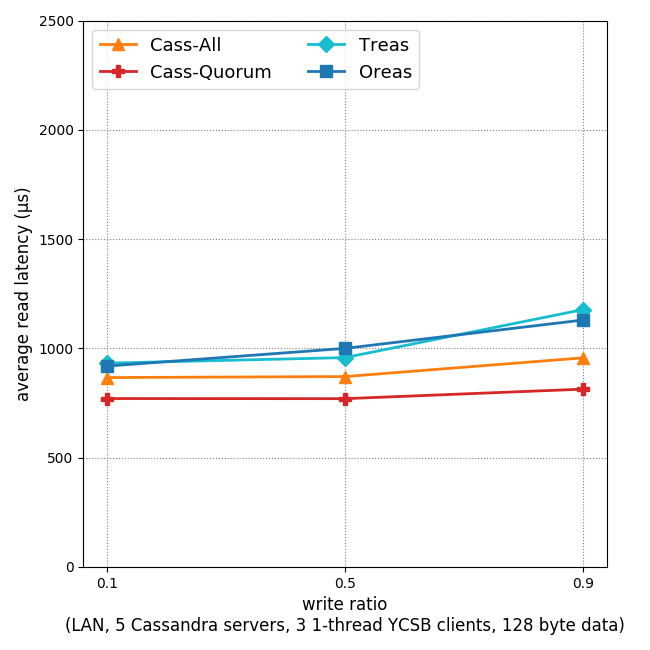
\includegraphics[width=0.9\linewidth]{img/LAN_7_latency,_vary_write,_5_svrs,_average_read.png}
		\caption{average read latency vs. write ratio}
		\label{fig:latency-read-ratio-avg}
	\end{subfigure}
	\hfill %%
	\begin{subfigure}[b]{0.32\textwidth}
		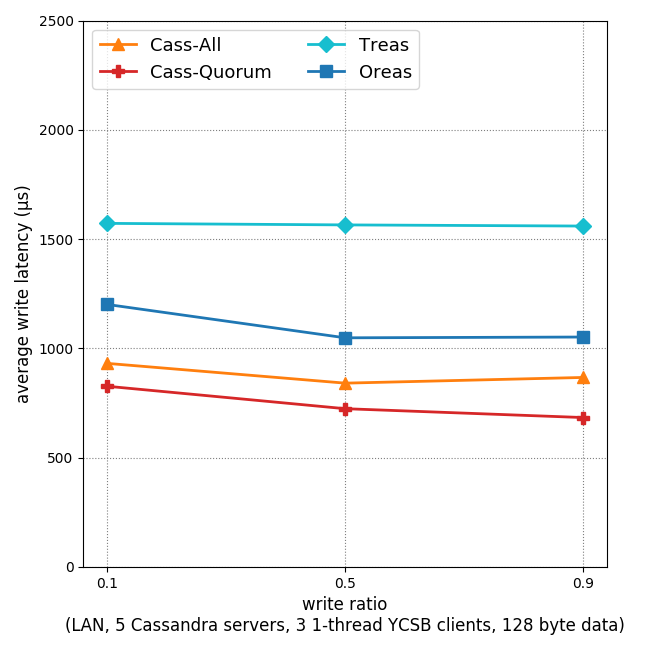
\includegraphics[width=0.9\linewidth]{img/LAN_9_latency,_vary_write,_5_svrs,_average_write.png}
		\caption{average write latency vs. write ratio}
		\label{fig:latency-write-ratio-avg}
	\end{subfigure}  
	\hfill %%
	\begin{subfigure}[b]{0.32\textwidth}
		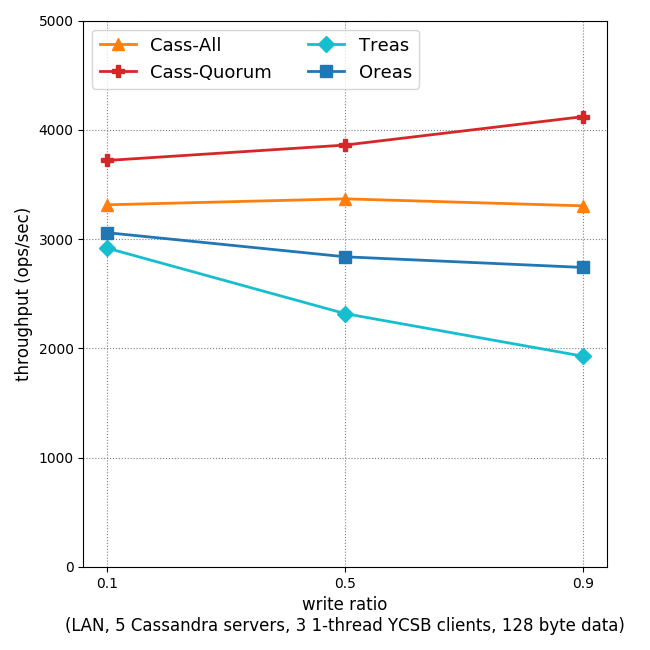
\includegraphics[width=0.9\linewidth]{img/LAN_6_throughput,_vary_write,_5_svrs.png}
		\caption{throughput vs. write ratio}
		\label{fig:throughput-ratio}
	\end{subfigure}

	\begin{subfigure}[b]{0.32\textwidth}
		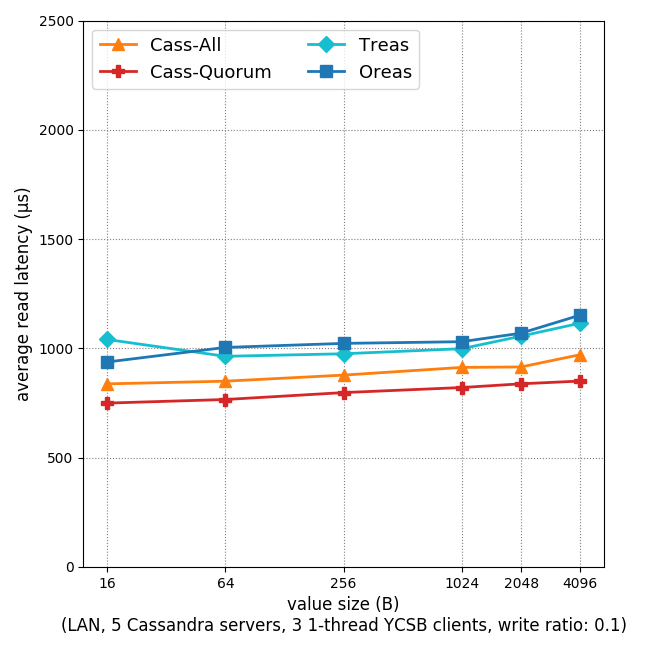
\includegraphics[width=0.9\linewidth]{img/LAN_12_latency,_vary_size,_5_svrs,_average_read.png}
		\caption{avg read latency vs. data size}
		\label{fig:latency-read-size-avg}
	\end{subfigure}    	
	\hfill
	\begin{subfigure}[b]{0.32\textwidth}
		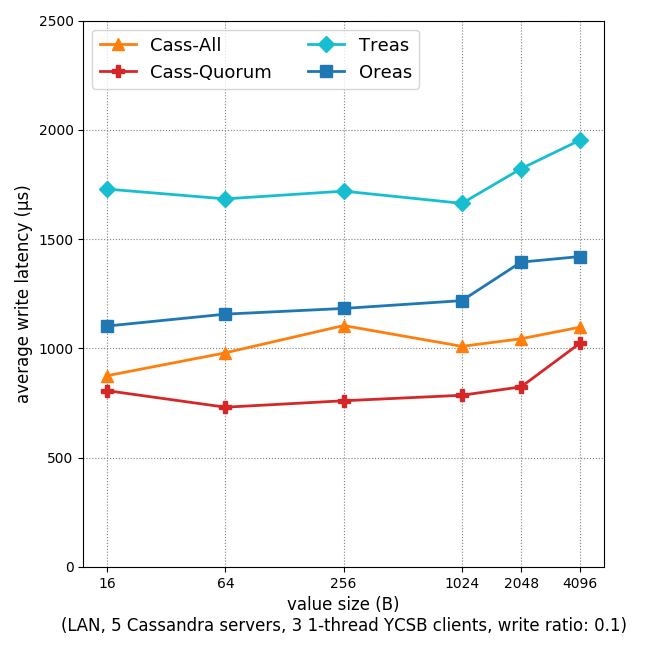
\includegraphics[width=0.9\linewidth]{img/LAN_14_latency,_vary_size,_5_svrs,_average_write.png}
		\caption{avg write latency vs. data size}
		\label{fig:latency-write-size-avg}
	\end{subfigure}    	
	\hfill %%	
	\begin{subfigure}[b]{0.32\textwidth}
		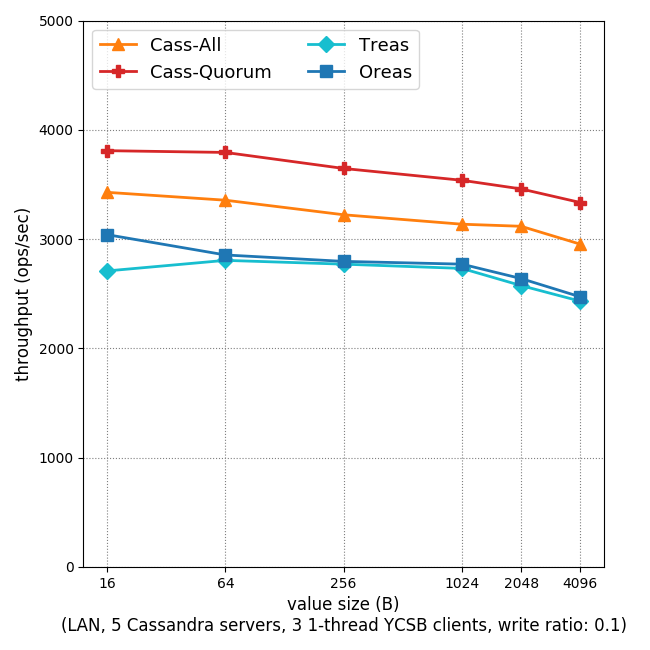
\includegraphics[width=0.9\linewidth]{img/LAN_11_throughput,_vary_size,_5_svrs.png}
		\caption{throughput vs. data size}
		\label{fig:throughput-size}
	\end{subfigure}    
	%	\hfill DON"T SHOW THIS ==> need to argue about inconsistent result for the %%%
	%	\begin{subfigure}[b]{0.3\textwidth}
	%		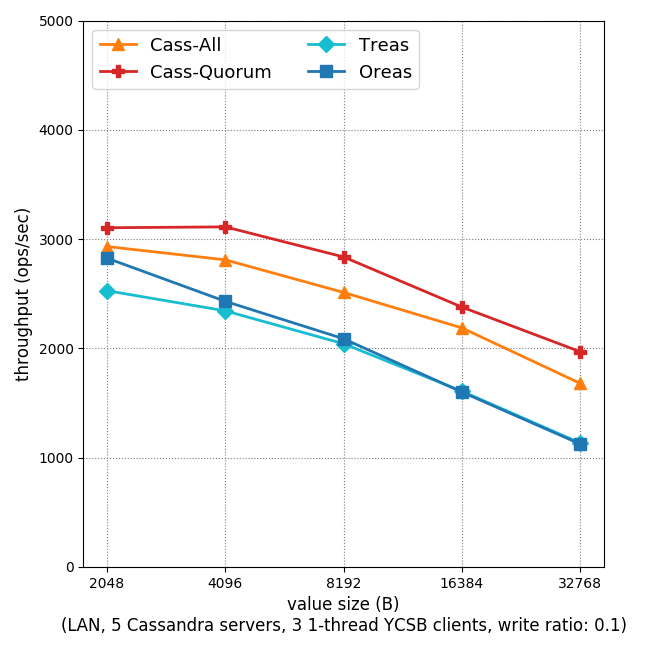
\includegraphics[width=0.9\linewidth]{img/LAN_16_throughput,_vary_size,_5_svrs.png}
	%		\caption{throughput vs. large data size}
	%		\label{fig:throughput-size-large}
	%	\end{subfigure}    	
	\caption{Comparison of latency and throughput of different configurations}\label{fig:evaluation}
\end{figure*}

%\section{CassandrEAS: Evaluation}
\subsection{Evaluation}
\label{s:evaluation}

We evaluate the performance of CassandrEAS by comparing it to the vanilla Cassandra (version 3.11). 
Cassandra-All requires the coordinator to hear from every server, whereas Cassandra-Quorum only requires to hear from a majority quorum of servers.

%and Cass-ABD. Cass-ABD replaced Cassandra's replication protocol with ABD \cite{ABD96}, which is a storage algorithm based on logical timestamps.
%We present the highlights of our evaluation results below:

%\begin{itemize}
%	\item \red{What should be here?}
%\end{itemize}

%\subsection{Experimental Setup}

%\paragraph{Cluster Configuration}
%\vspace*{3pt}
%\noindent\textbf{Cluster Configuration}~~
\paragraph*{Cluster Configuration and Workload}
We use the Google Cloud Platform (GCP) as our testing platform.
Each virtual machine (VM) is equipped with 4 virtual CPUs, 16 GB memory, and hosting Ubuntu 14.04 LTS.
All VMs are located in datacenter us-east1-c (South Carolina).
VMs use internal IP’s for communication.
The average RTT between any two VMs is around $0.3$ ms (based on issuing command for 30 seconds), and TCP bandwidth measured by Iperf is around $7.5$ Gbits/sec. %We use ping to estimate RTT.
For most of evaluation, our cluster consists of 5 VMs, and 3 YCSB single-threaded clients. Thus, $\delta = 3$.

%\paragraph{Workload}
%\vspace{3pt}
%\noindent\textbf{Workload}~~
%\subsection{Workload}
We use Yahoo! Cloud Serving Benchmark (YCSB) to generate realistic workload. We first insert a total of 30,000 KV-pairs, and each user performs 100,000 read or write operations. Recall that we have 3 YCSB clients, so we have 300,000 operations in total. We report the aggregated throughput, i.e., the sum of total operations per second across three YCSB clients. %We use the ``default Workload A'' provided by YCSB, whose operations follow Zipfian distribution.

%We use the Yahoo! Cloud Serving Benchmark (YCSB) \cite{YCSB} for evaluation. We did not choose Cassandra's own stress test tool, because it does not provide a straightforward way to disable Batch operation. Furthermore, it uses auto-generated data for all columns predefined.
%All of our YCSB workloads are modified from the ``default Workload A'' -- read-update workload. That is, YCSB first issues all-key insert before benchmarking, and we only benchmark on the read/update performances. 

%\vspace{3pt}
%\noindent\textbf{Performance}~~
\paragraph*{Performance}
Figure \ref{fig:evaluation} presents our evaluation results in different configurations.
Figures \ref{fig:latency-read-ratio-avg} to \ref{fig:throughput-ratio} show latency and throughput under different write ratio with data size equal to $128 B$. Read latency is comparable across all four algorithms. \treas{} has poor write latency due to the usage of logical timestamps, which requires an extra round-trip. \oreas{} has moderate penalty in write latency. 
Throughput is comparable in the case of write ratio $0.1$, a common case in NoSQL KV-stores.
Figures \ref{fig:latency-read-size-avg} to \ref{fig:throughput-size} show latency and throughput under different data size with write ratio $0.1$. We only show average latency, as 95 percentile has the same pattern.  Figure \ref{fig:throughput-size} demonstrates that CassandrEAS suffers moderate penalty on throughput.

%If we compare Figures \ref{fig:throughput-size} and \ref{fig:throughput-ratio}, then we see small discrepancy between throughput numbers. These two sets of experiments were conducted on different days. We have observed that performance can vary by around $10\%$ in different days with GCP. However, we are fairly confident that our evaluation methodology eliminates potential biases and noises. 

%Our evaluation results demonstrate that CassandrEAS provides latency and  throughput comparable to Cassandra in some cases. The average and 95 percentile latency numbers for reads and writes are shown in Fig~\ref{fig:evaluation} . The plots for throughput of operations under various value sizes and read to write frequency ratios further substantiates that there is no blocking operations due various workload properties. We obtained similar availablity and throughput results when we introduce server crashes. 

%\paragraph{Availability and Fault-tolerance}
%\vspace{3pt}
%\noindent\textbf{Aavailability and Fault-tolerance}~~
\paragraph*{Availability, Fault-tolerance, and Scalability}
CassandrEAS is highly available, fault-tolerant, and scalable, because its core is based on Cassandra.
It can continue serving client's operations as long as the conditions specified by $f$ and $\delta$ are satisfied.
We have tested our system with 7 servers and 1 crashed server, and observed minimal disruption on throughput (ranging from $0.1\%$ to $2.5\%$ decrease). We also observed that each YCSB client's throughput decreased a bit right after a server crashed, and later came back to normal throughput (compared with a cluster without any fault). Finally, we also tested clusters with 7, 9, and 11 servers. The throughput of \oreasSpace is in the range of $77 - 80 \%$ of Cassandra's. This demonstrates that CassandrEAS' performance is also scalable, i.e., the throughput increases when $n$ increases.
%some data with n=7, delta=3, 16B, w/r = 0.1
%name     throughput
%Treas-f=0 2682.11
%Treas-f=1 2610.55
%Oreas-f=0 2702.34
%Oreas-f=1 2697.6
%Indeed, the throughput just decreased a little bit. I also observed that the throughput at each YCSB client decreases 100-200 ops/sec for less than 10 seconds then comes back as normal.


\paragraph*{Correctness}
We develop a consistency checker based on the approach specified in \cite{Lynch1996} to ensure that our implementation also provides this guarantee. Validating strong consistency requires precise clock synchronization across all servers. %, since it needs to use global clock to ordering operations and events. 
This is impossible to achieve in a distributed system where clock drift is inevitable. To circumvent it, we deploy our CassandrEAS servers on a single machine and use Mininet \cite{MininetWebsite} to simulate the underlying network communication. Our checker then uses the machine time as the global clock. We collect multiple traces under different configurations with failures. The checker verifies that all traces we tested satisfy atomicity.


\section{Summary}

Strong consistency, storage efficiency, and availability are three key features for NoSQL KV-stores. We demonstrated that through  CassandrEAS -- erasure coding can be used to reduce storage cost while incurring moderate performance penalty. One interesting future work is to investigate how to apply \treasmod{} and \oreas{} in other NoSQL KV-stores.
	%\input{design-kmk-v1}
	%\input{evaluation}
	
	%\input{old}
	%\input{implementation}
	
	%-------------------------------------------------------------------------------
	%\section*{Availability}
	%-------------------------------------------------------------------------------
	
	%USENIX program committees give extra points to submissions that are backed by artifacts that are publicly available. If you made your code or data available, it's worth mentioning this fact in a dedicated section.
	
	%-------------------------------------------------------------------------------
	\bibliographystyle{plain}
	\bibliography{biblio,biblio1,newbft,DSM,BFTnitin,hotcloudadd}
	
	%%%%%%%%%%%%%%%%%%%%%%%%%%%%%%%%%%%%%%%%%%%%%%%%%%%%%%%%%%%%%%%%%%%%%%%%%%%%%%%%
\end{document}
%%%%%%%%%%%%%%%%%%%%%%%%%%%%%%%%%%%%%%%%%%%%%%%%%%%%%%%%%%%%%%%%%%%%%%%%%%%%%%%%

%%  LocalWords:  endnotes includegraphics fread ptr nobj noindent
%%  LocalWords:  pdflatex acks
